\documentclass[11pt,a4paper]{article}
% SHARED LaTeX SETUP FOR UP2 & UP3 PARALLEL WRITING
% This file contains all shared packages, macros, and notation for consistency

% ===================================================================
% ESSENTIAL PACKAGES (Identical for both papers)
% ===================================================================
\usepackage[utf8]{inputenc}
\usepackage[T1]{fontenc}
\usepackage{amsmath,amsfonts,amssymb,amsthm}
\usepackage{mathtools}
\usepackage{geometry}
\usepackage{hyperref}
\usepackage{cleveref}
\usepackage{enumitem}
\usepackage{booktabs}
\usepackage{graphicx}
\usepackage{natbib}
\usepackage{array}
\usepackage{multicol}
\usepackage{algorithm}
\usepackage{algpseudocode}
\usepackage{xcolor}

% Page geometry (consistent across papers)
\geometry{margin=1in}

% ===================================================================
% SHARED THEOREM ENVIRONMENTS
% ===================================================================
\newtheorem{theorem}{Theorem}[section]
\newtheorem{principle}{Theorem}[section]
\newtheorem{lemma}[theorem]{Lemma}
\newtheorem{corollary}[theorem]{Corollary}
\newtheorem{proposition}[theorem]{Proposition}
\newtheorem{definition}[theorem]{Definition}
\newtheorem{remark}[theorem]{Remark}
\newtheorem{assumption}[theorem]{Assumption}
\newtheorem{example}[theorem]{Example}
\newtheorem{hypothesis}[theorem]{Hypothesis}

% ===================================================================
% UNIFIED MATHEMATICAL NOTATION (CRITICAL FOR CONSISTENCY)
% ===================================================================

% Core competitive measurement parameters
\newcommand{\deltaval}{\delta}           % Performance difference (μ_A - μ_B)/σ_A
\newcommand{\kappaval}{\kappa}           % Variance ratio σ_B/σ_A  
\newcommand{\etaval}{\eta}               % Environmental noise ratio σ_η/σ_A

% Mahalanobis distance variants
\newcommand{\DM}{D_{\text{M}}}           % Basic Mahalanobis distance
\newcommand{\DMenv}{D_{\text{M}}^{(\text{env})}} % Environmental Mahalanobis distance

% Quadrant notation (consistent Q1-Q4 across papers)
\newcommand{\QOne}{Q_1}                  % Optimal quadrant
\newcommand{\QTwo}{Q_2}                  % Transitional quadrant  
\newcommand{\QThree}{Q_3}                % Inverse quadrant
\newcommand{\QFour}{Q_4}                 % Crisis/Extinct quadrant

% Performance measures
\newcommand{\Sth}{S_{\text{th}}}         % Theoretical separability
\newcommand{\Semp}{S_{\text{emp}}}       % Empirical separability
\newcommand{\Sabs}{S_{\text{abs}}}       % Absolute measure separability
\newcommand{\Srel}{S_{\text{rel}}}       % Relative measure separability

% Information and effect size measures
\newcommand{\Icontent}{I}                % Information content
\newcommand{\effectsize}{d}              % Effect size (Cohen's d relationship)

% Evolutionary fitness function (UP3 specific but referenced in UP2)
\newcommand{\Fitness}{F(\deltaval, \kappaval)} % Evolutionary fitness function
\newcommand{\FitnessQ}[1]{F_{Q_{#1}}}    % Quadrant-specific fitness

% Environmental integration formula (UP2 specific but referenced in UP3)
\newcommand{\SNRimprovement}{\text{SNR}_{\text{improvement}}}
\newcommand{\SNRformula}{\frac{1}{\sqrt{1 + \frac{2\etaval^2}{1 + \kappaval^2}}}}

% Statistical operators
\DeclareMathOperator{\sign}{sign}
\DeclareMathOperator{\Var}{Var}
\DeclareMathOperator{\Cov}{Cov}
\DeclareMathOperator{\E}{\mathbb{E}}
\DeclareMathOperator{\Prob}{\mathbb{P}}
\DeclareMathOperator*{\argmax}{arg\,max}
\DeclareMathOperator*{\argmin}{arg\,min}

% ===================================================================
% SHARED COLOR SCHEME (For consistent figures)
% ===================================================================
\definecolor{Q1color}{RGB}{0, 128, 0}    % Green for Q1 (Optimal)
\definecolor{Q2color}{RGB}{255, 165, 0}  % Orange for Q2 (Transitional)
\definecolor{Q3color}{RGB}{255, 0, 0}    % Red for Q3 (Inverse)
\definecolor{Q4color}{RGB}{128, 128, 128} % Gray for Q4 (Extinct)
\definecolor{envcolor}{RGB}{0, 0, 255}   % Blue for environmental effects

% ===================================================================
% CROSS-PAPER REFERENCE COMMANDS
% ===================================================================
% These will be updated with actual paper references once submitted
\newcommand{\paperone}{UP1}          % Reference to empirical relative measures paper
\newcommand{\papertwo}{UP2}        % Self-reference for UP2
\newcommand{\paperthree}{UP3}      % Self-reference for UP3
\newcommand{\paperfour}{UP4}       % Forward reference to temporal dynamics

% Cross-paper equation references (to be updated)
\newcommand{\DMformula}{\DM = \frac{|\deltaval|}{\sqrt{1 + \kappaval^2}}}
\newcommand{\DMenvformula}{\DMenv = \frac{|\deltaval|}{\sqrt{1 + \kappaval^2 + 2\etaval^2}}}
\newcommand{\Fitnessformula}{\Fitness = \begin{cases} 
    \deltaval \times (1 - \kappaval) & \text{if } \kappaval < 1 \\
    \deltaval \times (\kappaval - 1) & \text{if } \kappaval > 1 
\end{cases}}

% ===================================================================
% SHARED MACROS FOR RESULTS PRESENTATION
% ===================================================================
\newcommand{\correlationUPTwo}{r = 0.973}        % UP2 SVM correlation
\newcommand{\correlationUPThree}{r = 0.912}      % UP3 theory-data correlation
\newcommand{\SNRresult}{53.2\%}                  % UP2 SNR improvement result
\newcommand{\QFourextinction}{0}                 % UP3 Q4 extinction result (0 datasets)
\newcommand{\parametercount}{644}                % Total parameter combinations tested
\newcommand{\domaincount}{5}                     % Cross-domain validation count

% ===================================================================
% FIGURE AND TABLE FORMATTING (Consistent style)
% ===================================================================
% Standard figure width for consistency
\newcommand{\figwidth}{0.8\textwidth}
\newcommand{\smallfigwidth}{0.6\textwidth}

% Table formatting for results
\newcommand{\resultscaption}[1]{\caption{#1}}
\newcommand{\validationtable}{\begin{tabular}{lccc} \toprule}
%\newcommand{\endvalidationtable}{\bottomrule \end{tabular}}

% ===================================================================
% JOURNAL-SPECIFIC FORMATTING FLAGS
% ===================================================================
% These can be toggled based on target journal requirements
\newif\ifNatureformat\Natureformatfalse       % Nature family journals
\newif\ifIEEEformat\IEEEformatfalse           % IEEE journals
\newif\ifJMLRformat\JMLRformatfalse           % JMLR format
\newif\ifPLOSformat\PLOSformatfalse           % PLOS family

% ===================================================================
% SHARED ABSTRACT COMPONENTS
% ===================================================================
% Keywords that should appear in both papers for consistency
\newcommand{\sharedkeywords}{competitive measurement, Mahalanobis distance, asymmetric analysis, quadrant classification}

% Common background statement for both papers
\newcommand{\competitivemeasurement}{Competitive measurement between entities A and B represents a fundamental challenge across domains from financial analysis to clinical research}

% Common framework reference
\newcommand{\frameworkfoundation}{Building on the empirical success of relative measures $R = X_A - X_B$ established in \paperone}

% ===================================================================
% VALIDATION RESULT FORMATTING
% ===================================================================
\newcommand{\validationresult}[3]{%
  \textbf{#1}: #2 (#3)%
}

\newcommand{\quadrantresult}[4]{%
  \textbf{#1} ($\deltaval #2 0, \kappaval #3 1$): #4%
}

% ===================================================================
% MANUSCRIPT STRUCTURE CONSISTENCY
% ===================================================================
% Ensure both papers follow the same high-level structure
\newcommand{\abstractlength}{150 words}
\newcommand{\introductionlength}{1.5 pages}
\newcommand{\theorylength}{3 pages}
\newcommand{\resultslength}{2.5 pages}
\newcommand{\discussionlength}{1 page}

% ===================================================================
% DEBUGGING AND CONSISTENCY CHECKS
% ===================================================================
% Commands to verify cross-paper consistency during writing
\newcommand{\consistencycheck}[1]{\textcolor{red}{CHECK: #1}}
\newcommand{\crossref}[1]{\textcolor{blue}{CROSSREF: #1}}
\newcommand{\needsupdate}[1]{\textcolor{orange}{UPDATE: #1}}

% Remove these in final version by redefining as empty
% \renewcommand{\consistencycheck}[1]{}
% \renewcommand{\crossref}[1]{}
% \renewcommand{\needsupdate}[1]{}

% ===================================================================
% AUTHOR INFORMATION TEMPLATE
% ===================================================================
\newcommand{\authorone}{M.R. Brown\thanks{Corresponding author. Email: m.r.brown@swansea.ac.uk}}
\newcommand{\authortwo}{Author 2}
\newcommand{\authorthree}{Author 3}

\newcommand{\affiliationone}{Department of Applied Mathematics, Swansea University}
\newcommand{\affiliationtwo}{Department of Statistics, University Name}  
\newcommand{\affiliationthree}{Department of Business Analytics, University Name}

% ===================================================================
% USAGE INSTRUCTIONS
% ===================================================================
% Include this file in both UP2 and UP3 manuscripts with:
% % SHARED LaTeX SETUP FOR UP2 & UP3 PARALLEL WRITING
% This file contains all shared packages, macros, and notation for consistency

% ===================================================================
% ESSENTIAL PACKAGES (Identical for both papers)
% ===================================================================
\usepackage[utf8]{inputenc}
\usepackage[T1]{fontenc}
\usepackage{amsmath,amsfonts,amssymb,amsthm}
\usepackage{mathtools}
\usepackage{geometry}
\usepackage{hyperref}
\usepackage{cleveref}
\usepackage{enumitem}
\usepackage{booktabs}
\usepackage{graphicx}
\usepackage{natbib}
\usepackage{array}
\usepackage{multicol}
\usepackage{algorithm}
\usepackage{algpseudocode}
\usepackage{xcolor}

% Page geometry (consistent across papers)
\geometry{margin=1in}

% ===================================================================
% SHARED THEOREM ENVIRONMENTS
% ===================================================================
\newtheorem{theorem}{Theorem}[section]
\newtheorem{principle}{Theorem}[section]
\newtheorem{lemma}[theorem]{Lemma}
\newtheorem{corollary}[theorem]{Corollary}
\newtheorem{proposition}[theorem]{Proposition}
\newtheorem{definition}[theorem]{Definition}
\newtheorem{remark}[theorem]{Remark}
\newtheorem{assumption}[theorem]{Assumption}
\newtheorem{example}[theorem]{Example}
\newtheorem{hypothesis}[theorem]{Hypothesis}

% ===================================================================
% UNIFIED MATHEMATICAL NOTATION (CRITICAL FOR CONSISTENCY)
% ===================================================================

% Core competitive measurement parameters
\newcommand{\deltaval}{\delta}           % Performance difference (μ_A - μ_B)/σ_A
\newcommand{\kappaval}{\kappa}           % Variance ratio σ_B/σ_A  
\newcommand{\etaval}{\eta}               % Environmental noise ratio σ_η/σ_A

% Mahalanobis distance variants
\newcommand{\DM}{D_{\text{M}}}           % Basic Mahalanobis distance
\newcommand{\DMenv}{D_{\text{M}}^{(\text{env})}} % Environmental Mahalanobis distance

% Quadrant notation (consistent Q1-Q4 across papers)
\newcommand{\QOne}{Q_1}                  % Optimal quadrant
\newcommand{\QTwo}{Q_2}                  % Transitional quadrant  
\newcommand{\QThree}{Q_3}                % Inverse quadrant
\newcommand{\QFour}{Q_4}                 % Crisis/Extinct quadrant

% Performance measures
\newcommand{\Sth}{S_{\text{th}}}         % Theoretical separability
\newcommand{\Semp}{S_{\text{emp}}}       % Empirical separability
\newcommand{\Sabs}{S_{\text{abs}}}       % Absolute measure separability
\newcommand{\Srel}{S_{\text{rel}}}       % Relative measure separability

% Information and effect size measures
\newcommand{\Icontent}{I}                % Information content
\newcommand{\effectsize}{d}              % Effect size (Cohen's d relationship)

% Evolutionary fitness function (UP3 specific but referenced in UP2)
\newcommand{\Fitness}{F(\deltaval, \kappaval)} % Evolutionary fitness function
\newcommand{\FitnessQ}[1]{F_{Q_{#1}}}    % Quadrant-specific fitness

% Environmental integration formula (UP2 specific but referenced in UP3)
\newcommand{\SNRimprovement}{\text{SNR}_{\text{improvement}}}
\newcommand{\SNRformula}{\frac{1}{\sqrt{1 + \frac{2\etaval^2}{1 + \kappaval^2}}}}

% Statistical operators
\DeclareMathOperator{\sign}{sign}
\DeclareMathOperator{\Var}{Var}
\DeclareMathOperator{\Cov}{Cov}
\DeclareMathOperator{\E}{\mathbb{E}}
\DeclareMathOperator{\Prob}{\mathbb{P}}
\DeclareMathOperator*{\argmax}{arg\,max}
\DeclareMathOperator*{\argmin}{arg\,min}

% ===================================================================
% SHARED COLOR SCHEME (For consistent figures)
% ===================================================================
\definecolor{Q1color}{RGB}{0, 128, 0}    % Green for Q1 (Optimal)
\definecolor{Q2color}{RGB}{255, 165, 0}  % Orange for Q2 (Transitional)
\definecolor{Q3color}{RGB}{255, 0, 0}    % Red for Q3 (Inverse)
\definecolor{Q4color}{RGB}{128, 128, 128} % Gray for Q4 (Extinct)
\definecolor{envcolor}{RGB}{0, 0, 255}   % Blue for environmental effects

% ===================================================================
% CROSS-PAPER REFERENCE COMMANDS
% ===================================================================
% These will be updated with actual paper references once submitted
\newcommand{\paperone}{UP1}          % Reference to empirical relative measures paper
\newcommand{\papertwo}{UP2}        % Self-reference for UP2
\newcommand{\paperthree}{UP3}      % Self-reference for UP3
\newcommand{\paperfour}{UP4}       % Forward reference to temporal dynamics

% Cross-paper equation references (to be updated)
\newcommand{\DMformula}{\DM = \frac{|\deltaval|}{\sqrt{1 + \kappaval^2}}}
\newcommand{\DMenvformula}{\DMenv = \frac{|\deltaval|}{\sqrt{1 + \kappaval^2 + 2\etaval^2}}}
\newcommand{\Fitnessformula}{\Fitness = \begin{cases} 
    \deltaval \times (1 - \kappaval) & \text{if } \kappaval < 1 \\
    \deltaval \times (\kappaval - 1) & \text{if } \kappaval > 1 
\end{cases}}

% ===================================================================
% SHARED MACROS FOR RESULTS PRESENTATION
% ===================================================================
\newcommand{\correlationUPTwo}{r = 0.973}        % UP2 SVM correlation
\newcommand{\correlationUPThree}{r = 0.912}      % UP3 theory-data correlation
\newcommand{\SNRresult}{53.2\%}                  % UP2 SNR improvement result
\newcommand{\QFourextinction}{0}                 % UP3 Q4 extinction result (0 datasets)
\newcommand{\parametercount}{644}                % Total parameter combinations tested
\newcommand{\domaincount}{5}                     % Cross-domain validation count

% ===================================================================
% FIGURE AND TABLE FORMATTING (Consistent style)
% ===================================================================
% Standard figure width for consistency
\newcommand{\figwidth}{0.8\textwidth}
\newcommand{\smallfigwidth}{0.6\textwidth}

% Table formatting for results
\newcommand{\resultscaption}[1]{\caption{#1}}
\newcommand{\validationtable}{\begin{tabular}{lccc} \toprule}
%\newcommand{\endvalidationtable}{\bottomrule \end{tabular}}

% ===================================================================
% JOURNAL-SPECIFIC FORMATTING FLAGS
% ===================================================================
% These can be toggled based on target journal requirements
\newif\ifNatureformat\Natureformatfalse       % Nature family journals
\newif\ifIEEEformat\IEEEformatfalse           % IEEE journals
\newif\ifJMLRformat\JMLRformatfalse           % JMLR format
\newif\ifPLOSformat\PLOSformatfalse           % PLOS family

% ===================================================================
% SHARED ABSTRACT COMPONENTS
% ===================================================================
% Keywords that should appear in both papers for consistency
\newcommand{\sharedkeywords}{competitive measurement, Mahalanobis distance, asymmetric analysis, quadrant classification}

% Common background statement for both papers
\newcommand{\competitivemeasurement}{Competitive measurement between entities A and B represents a fundamental challenge across domains from financial analysis to clinical research}

% Common framework reference
\newcommand{\frameworkfoundation}{Building on the empirical success of relative measures $R = X_A - X_B$ established in \paperone}

% ===================================================================
% VALIDATION RESULT FORMATTING
% ===================================================================
\newcommand{\validationresult}[3]{%
  \textbf{#1}: #2 (#3)%
}

\newcommand{\quadrantresult}[4]{%
  \textbf{#1} ($\deltaval #2 0, \kappaval #3 1$): #4%
}

% ===================================================================
% MANUSCRIPT STRUCTURE CONSISTENCY
% ===================================================================
% Ensure both papers follow the same high-level structure
\newcommand{\abstractlength}{150 words}
\newcommand{\introductionlength}{1.5 pages}
\newcommand{\theorylength}{3 pages}
\newcommand{\resultslength}{2.5 pages}
\newcommand{\discussionlength}{1 page}

% ===================================================================
% DEBUGGING AND CONSISTENCY CHECKS
% ===================================================================
% Commands to verify cross-paper consistency during writing
\newcommand{\consistencycheck}[1]{\textcolor{red}{CHECK: #1}}
\newcommand{\crossref}[1]{\textcolor{blue}{CROSSREF: #1}}
\newcommand{\needsupdate}[1]{\textcolor{orange}{UPDATE: #1}}

% Remove these in final version by redefining as empty
% \renewcommand{\consistencycheck}[1]{}
% \renewcommand{\crossref}[1]{}
% \renewcommand{\needsupdate}[1]{}

% ===================================================================
% AUTHOR INFORMATION TEMPLATE
% ===================================================================
\newcommand{\authorone}{M.R. Brown\thanks{Corresponding author. Email: m.r.brown@swansea.ac.uk}}
\newcommand{\authortwo}{Author 2}
\newcommand{\authorthree}{Author 3}

\newcommand{\affiliationone}{Department of Applied Mathematics, Swansea University}
\newcommand{\affiliationtwo}{Department of Statistics, University Name}  
\newcommand{\affiliationthree}{Department of Business Analytics, University Name}

% ===================================================================
% USAGE INSTRUCTIONS
% ===================================================================
% Include this file in both UP2 and UP3 manuscripts with:
% % SHARED LaTeX SETUP FOR UP2 & UP3 PARALLEL WRITING
% This file contains all shared packages, macros, and notation for consistency

% ===================================================================
% ESSENTIAL PACKAGES (Identical for both papers)
% ===================================================================
\usepackage[utf8]{inputenc}
\usepackage[T1]{fontenc}
\usepackage{amsmath,amsfonts,amssymb,amsthm}
\usepackage{mathtools}
\usepackage{geometry}
\usepackage{hyperref}
\usepackage{cleveref}
\usepackage{enumitem}
\usepackage{booktabs}
\usepackage{graphicx}
\usepackage{natbib}
\usepackage{array}
\usepackage{multicol}
\usepackage{algorithm}
\usepackage{algpseudocode}
\usepackage{xcolor}

% Page geometry (consistent across papers)
\geometry{margin=1in}

% ===================================================================
% SHARED THEOREM ENVIRONMENTS
% ===================================================================
\newtheorem{theorem}{Theorem}[section]
\newtheorem{principle}{Theorem}[section]
\newtheorem{lemma}[theorem]{Lemma}
\newtheorem{corollary}[theorem]{Corollary}
\newtheorem{proposition}[theorem]{Proposition}
\newtheorem{definition}[theorem]{Definition}
\newtheorem{remark}[theorem]{Remark}
\newtheorem{assumption}[theorem]{Assumption}
\newtheorem{example}[theorem]{Example}
\newtheorem{hypothesis}[theorem]{Hypothesis}

% ===================================================================
% UNIFIED MATHEMATICAL NOTATION (CRITICAL FOR CONSISTENCY)
% ===================================================================

% Core competitive measurement parameters
\newcommand{\deltaval}{\delta}           % Performance difference (μ_A - μ_B)/σ_A
\newcommand{\kappaval}{\kappa}           % Variance ratio σ_B/σ_A  
\newcommand{\etaval}{\eta}               % Environmental noise ratio σ_η/σ_A

% Mahalanobis distance variants
\newcommand{\DM}{D_{\text{M}}}           % Basic Mahalanobis distance
\newcommand{\DMenv}{D_{\text{M}}^{(\text{env})}} % Environmental Mahalanobis distance

% Quadrant notation (consistent Q1-Q4 across papers)
\newcommand{\QOne}{Q_1}                  % Optimal quadrant
\newcommand{\QTwo}{Q_2}                  % Transitional quadrant  
\newcommand{\QThree}{Q_3}                % Inverse quadrant
\newcommand{\QFour}{Q_4}                 % Crisis/Extinct quadrant

% Performance measures
\newcommand{\Sth}{S_{\text{th}}}         % Theoretical separability
\newcommand{\Semp}{S_{\text{emp}}}       % Empirical separability
\newcommand{\Sabs}{S_{\text{abs}}}       % Absolute measure separability
\newcommand{\Srel}{S_{\text{rel}}}       % Relative measure separability

% Information and effect size measures
\newcommand{\Icontent}{I}                % Information content
\newcommand{\effectsize}{d}              % Effect size (Cohen's d relationship)

% Evolutionary fitness function (UP3 specific but referenced in UP2)
\newcommand{\Fitness}{F(\deltaval, \kappaval)} % Evolutionary fitness function
\newcommand{\FitnessQ}[1]{F_{Q_{#1}}}    % Quadrant-specific fitness

% Environmental integration formula (UP2 specific but referenced in UP3)
\newcommand{\SNRimprovement}{\text{SNR}_{\text{improvement}}}
\newcommand{\SNRformula}{\frac{1}{\sqrt{1 + \frac{2\etaval^2}{1 + \kappaval^2}}}}

% Statistical operators
\DeclareMathOperator{\sign}{sign}
\DeclareMathOperator{\Var}{Var}
\DeclareMathOperator{\Cov}{Cov}
\DeclareMathOperator{\E}{\mathbb{E}}
\DeclareMathOperator{\Prob}{\mathbb{P}}
\DeclareMathOperator*{\argmax}{arg\,max}
\DeclareMathOperator*{\argmin}{arg\,min}

% ===================================================================
% SHARED COLOR SCHEME (For consistent figures)
% ===================================================================
\definecolor{Q1color}{RGB}{0, 128, 0}    % Green for Q1 (Optimal)
\definecolor{Q2color}{RGB}{255, 165, 0}  % Orange for Q2 (Transitional)
\definecolor{Q3color}{RGB}{255, 0, 0}    % Red for Q3 (Inverse)
\definecolor{Q4color}{RGB}{128, 128, 128} % Gray for Q4 (Extinct)
\definecolor{envcolor}{RGB}{0, 0, 255}   % Blue for environmental effects

% ===================================================================
% CROSS-PAPER REFERENCE COMMANDS
% ===================================================================
% These will be updated with actual paper references once submitted
\newcommand{\paperone}{UP1}          % Reference to empirical relative measures paper
\newcommand{\papertwo}{UP2}        % Self-reference for UP2
\newcommand{\paperthree}{UP3}      % Self-reference for UP3
\newcommand{\paperfour}{UP4}       % Forward reference to temporal dynamics

% Cross-paper equation references (to be updated)
\newcommand{\DMformula}{\DM = \frac{|\deltaval|}{\sqrt{1 + \kappaval^2}}}
\newcommand{\DMenvformula}{\DMenv = \frac{|\deltaval|}{\sqrt{1 + \kappaval^2 + 2\etaval^2}}}
\newcommand{\Fitnessformula}{\Fitness = \begin{cases} 
    \deltaval \times (1 - \kappaval) & \text{if } \kappaval < 1 \\
    \deltaval \times (\kappaval - 1) & \text{if } \kappaval > 1 
\end{cases}}

% ===================================================================
% SHARED MACROS FOR RESULTS PRESENTATION
% ===================================================================
\newcommand{\correlationUPTwo}{r = 0.973}        % UP2 SVM correlation
\newcommand{\correlationUPThree}{r = 0.912}      % UP3 theory-data correlation
\newcommand{\SNRresult}{53.2\%}                  % UP2 SNR improvement result
\newcommand{\QFourextinction}{0}                 % UP3 Q4 extinction result (0 datasets)
\newcommand{\parametercount}{644}                % Total parameter combinations tested
\newcommand{\domaincount}{5}                     % Cross-domain validation count

% ===================================================================
% FIGURE AND TABLE FORMATTING (Consistent style)
% ===================================================================
% Standard figure width for consistency
\newcommand{\figwidth}{0.8\textwidth}
\newcommand{\smallfigwidth}{0.6\textwidth}

% Table formatting for results
\newcommand{\resultscaption}[1]{\caption{#1}}
\newcommand{\validationtable}{\begin{tabular}{lccc} \toprule}
%\newcommand{\endvalidationtable}{\bottomrule \end{tabular}}

% ===================================================================
% JOURNAL-SPECIFIC FORMATTING FLAGS
% ===================================================================
% These can be toggled based on target journal requirements
\newif\ifNatureformat\Natureformatfalse       % Nature family journals
\newif\ifIEEEformat\IEEEformatfalse           % IEEE journals
\newif\ifJMLRformat\JMLRformatfalse           % JMLR format
\newif\ifPLOSformat\PLOSformatfalse           % PLOS family

% ===================================================================
% SHARED ABSTRACT COMPONENTS
% ===================================================================
% Keywords that should appear in both papers for consistency
\newcommand{\sharedkeywords}{competitive measurement, Mahalanobis distance, asymmetric analysis, quadrant classification}

% Common background statement for both papers
\newcommand{\competitivemeasurement}{Competitive measurement between entities A and B represents a fundamental challenge across domains from financial analysis to clinical research}

% Common framework reference
\newcommand{\frameworkfoundation}{Building on the empirical success of relative measures $R = X_A - X_B$ established in \paperone}

% ===================================================================
% VALIDATION RESULT FORMATTING
% ===================================================================
\newcommand{\validationresult}[3]{%
  \textbf{#1}: #2 (#3)%
}

\newcommand{\quadrantresult}[4]{%
  \textbf{#1} ($\deltaval #2 0, \kappaval #3 1$): #4%
}

% ===================================================================
% MANUSCRIPT STRUCTURE CONSISTENCY
% ===================================================================
% Ensure both papers follow the same high-level structure
\newcommand{\abstractlength}{150 words}
\newcommand{\introductionlength}{1.5 pages}
\newcommand{\theorylength}{3 pages}
\newcommand{\resultslength}{2.5 pages}
\newcommand{\discussionlength}{1 page}

% ===================================================================
% DEBUGGING AND CONSISTENCY CHECKS
% ===================================================================
% Commands to verify cross-paper consistency during writing
\newcommand{\consistencycheck}[1]{\textcolor{red}{CHECK: #1}}
\newcommand{\crossref}[1]{\textcolor{blue}{CROSSREF: #1}}
\newcommand{\needsupdate}[1]{\textcolor{orange}{UPDATE: #1}}

% Remove these in final version by redefining as empty
% \renewcommand{\consistencycheck}[1]{}
% \renewcommand{\crossref}[1]{}
% \renewcommand{\needsupdate}[1]{}

% ===================================================================
% AUTHOR INFORMATION TEMPLATE
% ===================================================================
\newcommand{\authorone}{M.R. Brown\thanks{Corresponding author. Email: m.r.brown@swansea.ac.uk}}
\newcommand{\authortwo}{Author 2}
\newcommand{\authorthree}{Author 3}

\newcommand{\affiliationone}{Department of Applied Mathematics, Swansea University}
\newcommand{\affiliationtwo}{Department of Statistics, University Name}  
\newcommand{\affiliationthree}{Department of Business Analytics, University Name}

% ===================================================================
% USAGE INSTRUCTIONS
% ===================================================================
% Include this file in both UP2 and UP3 manuscripts with:
% \input{shared_latex_setup}
% 
% This ensures perfect consistency in:
% - Mathematical notation (δ, κ, η, D_M, etc.)
% - Quadrant references (Q1, Q2, Q3, Q4)
% - Cross-paper citations
% - Figure and table formatting
% - Color schemes for visualizations
% - Statistical result presentation
%
% Update the cross-references and journal formatting flags as needed
% for specific submission targets.



% ===================================================================
% PAPER-SPECIFIC METADATA (Add to existing file)
% ===================================================================
\newcommand{\UPOneTitle}{Environmental Noise Cancellation in Competitive Measurement}
\newcommand{\UPTwoTitle}{Asymmetric Mahalanobis Framework for Competitive Measurement}
\newcommand{\UPThreeTitle}{Evolutionary Extinction Theory in Competitive Measurement}
\newcommand{\UPFourTitle}{Temporal Dynamics in Competitive Measurement}

% Abstract word counts for consistency checking
\newcommand{\abstractwordcount}{150}
\newcommand{\checkabstractlength}[1]{%
  \immediate\write16{Abstract length: #1 words (target: \abstractwordcount)}%
}

% ===================================================================
% CROSS-PAPER CITATION COMMANDS
% ===================================================================
\newcommand{\citeUPOne}{\cite{UP1}}      % Will be updated with actual citations
\newcommand{\citeUPTwo}{\cite{UP2}}
\newcommand{\citeUPThree}{\cite{UP3}}
\newcommand{\citeUPFour}{\cite{UP4}}

% Equation references across papers
\newcommand{\eqnSNRimprovement}{Equation (17) in \paperone}
\newcommand{\eqnMahalanobis}{Equation (12) in \papertwo}
\newcommand{\eqnFitness}{Equation (8) in \paperthree}

% ===================================================================
% RESULT FORMATTING CONSISTENCY
% ===================================================================
\newcommand{\resultformat}[2]{\textbf{#1:} #2}
\newcommand{\correlationformat}[1]{$r = #1$}
\newcommand{\percentformat}[1]{#1\%}
\newcommand{\significanceformat}[1]{$p < #1$}

% ===================================================================
% FIGURE CAPTION TEMPLATES
% ===================================================================
\newcommand{\quadrantfigcaption}{Four-quadrant classification of competitive scenarios showing the relationship between performance difference ($\deltaval$) and variance asymmetry ($\kappaval$)}

\newcommand{\validationfigcaption}{Theoretical vs. empirical validation showing strong correlation between framework predictions and observed results across multiple domains}
% 
% This ensures perfect consistency in:
% - Mathematical notation (δ, κ, η, D_M, etc.)
% - Quadrant references (Q1, Q2, Q3, Q4)
% - Cross-paper citations
% - Figure and table formatting
% - Color schemes for visualizations
% - Statistical result presentation
%
% Update the cross-references and journal formatting flags as needed
% for specific submission targets.



% ===================================================================
% PAPER-SPECIFIC METADATA (Add to existing file)
% ===================================================================
\newcommand{\UPOneTitle}{Environmental Noise Cancellation in Competitive Measurement}
\newcommand{\UPTwoTitle}{Asymmetric Mahalanobis Framework for Competitive Measurement}
\newcommand{\UPThreeTitle}{Evolutionary Extinction Theory in Competitive Measurement}
\newcommand{\UPFourTitle}{Temporal Dynamics in Competitive Measurement}

% Abstract word counts for consistency checking
\newcommand{\abstractwordcount}{150}
\newcommand{\checkabstractlength}[1]{%
  \immediate\write16{Abstract length: #1 words (target: \abstractwordcount)}%
}

% ===================================================================
% CROSS-PAPER CITATION COMMANDS
% ===================================================================
\newcommand{\citeUPOne}{\cite{UP1}}      % Will be updated with actual citations
\newcommand{\citeUPTwo}{\cite{UP2}}
\newcommand{\citeUPThree}{\cite{UP3}}
\newcommand{\citeUPFour}{\cite{UP4}}

% Equation references across papers
\newcommand{\eqnSNRimprovement}{Equation (17) in \paperone}
\newcommand{\eqnMahalanobis}{Equation (12) in \papertwo}
\newcommand{\eqnFitness}{Equation (8) in \paperthree}

% ===================================================================
% RESULT FORMATTING CONSISTENCY
% ===================================================================
\newcommand{\resultformat}[2]{\textbf{#1:} #2}
\newcommand{\correlationformat}[1]{$r = #1$}
\newcommand{\percentformat}[1]{#1\%}
\newcommand{\significanceformat}[1]{$p < #1$}

% ===================================================================
% FIGURE CAPTION TEMPLATES
% ===================================================================
\newcommand{\quadrantfigcaption}{Four-quadrant classification of competitive scenarios showing the relationship between performance difference ($\deltaval$) and variance asymmetry ($\kappaval$)}

\newcommand{\validationfigcaption}{Theoretical vs. empirical validation showing strong correlation between framework predictions and observed results across multiple domains}
% 
% This ensures perfect consistency in:
% - Mathematical notation (δ, κ, η, D_M, etc.)
% - Quadrant references (Q1, Q2, Q3, Q4)
% - Cross-paper citations
% - Figure and table formatting
% - Color schemes for visualizations
% - Statistical result presentation
%
% Update the cross-references and journal formatting flags as needed
% for specific submission targets.



% ===================================================================
% PAPER-SPECIFIC METADATA (Add to existing file)
% ===================================================================
\newcommand{\UPOneTitle}{Environmental Noise Cancellation in Competitive Measurement}
\newcommand{\UPTwoTitle}{Asymmetric Mahalanobis Framework for Competitive Measurement}
\newcommand{\UPThreeTitle}{Evolutionary Extinction Theory in Competitive Measurement}
\newcommand{\UPFourTitle}{Temporal Dynamics in Competitive Measurement}

% Abstract word counts for consistency checking
\newcommand{\abstractwordcount}{150}
\newcommand{\checkabstractlength}[1]{%
  \immediate\write16{Abstract length: #1 words (target: \abstractwordcount)}%
}

% ===================================================================
% CROSS-PAPER CITATION COMMANDS
% ===================================================================
\newcommand{\citeUPOne}{\cite{UP1}}      % Will be updated with actual citations
\newcommand{\citeUPTwo}{\cite{UP2}}
\newcommand{\citeUPThree}{\cite{UP3}}
\newcommand{\citeUPFour}{\cite{UP4}}

% Equation references across papers
\newcommand{\eqnSNRimprovement}{Equation (17) in \paperone}
\newcommand{\eqnMahalanobis}{Equation (12) in \papertwo}
\newcommand{\eqnFitness}{Equation (8) in \paperthree}

% ===================================================================
% RESULT FORMATTING CONSISTENCY
% ===================================================================
\newcommand{\resultformat}[2]{\textbf{#1:} #2}
\newcommand{\correlationformat}[1]{$r = #1$}
\newcommand{\percentformat}[1]{#1\%}
\newcommand{\significanceformat}[1]{$p < #1$}

% ===================================================================
% FIGURE CAPTION TEMPLATES
% ===================================================================
\newcommand{\quadrantfigcaption}{Four-quadrant classification of competitive scenarios showing the relationship between performance difference ($\deltaval$) and variance asymmetry ($\kappaval$)}

\newcommand{\validationfigcaption}{Theoretical vs. empirical validation showing strong correlation between framework predictions and observed results across multiple domains}

\title{Relative Advantage: Quantifying Performance in Noisy Competitive Settings}

\author{
    \authorone \\
    \textit{\affiliationone}
}
\date{\today}

\begin{document}
\maketitle

% ===================================================================
% UP1 ABSTRACT (150 words)
% ===================================================================
\begin{abstract}
\competitivemeasurement\ across domains from manufacturing to finance, yet traditional absolute measurements suffer from environmental noise contamination that obscures true competitive differences. We establish the theoretical foundation for relative measurement through systematic environmental noise cancellation, demonstrating why $R = X_A - X_B$ achieves superior signal-to-noise ratios compared to independent absolute measurements. Our framework reveals that simultaneous measurement enables complete environmental factor elimination, yielding SNR improvements of $1 + 2\sigma_\eta^2/(\sigma_A^2 + \sigma_B^2)$ over traditional approaches. Through comprehensive empirical validation across manufacturing, financial, and healthcare domains, we demonstrate correlation coefficients exceeding 0.91 between theoretical predictions and observed performance improvements. The framework establishes three complementary metrics—separability, information content, and effect size—that translate SNR improvements into actionable competitive intelligence. This foundational work enables principled competitive measurement design while establishing the theoretical basis for advanced asymmetric and temporal extensions.

\textbf{Keywords:} competitive measurement, environmental noise, signal-to-noise ratio, relative measurement, performance metrics
\end{abstract}

% ===================================================================
% MAIN SECTIONS
% ===================================================================
\section{Introduction}

Across competitive measurement contexts, from sports performance analysis to financial portfolio management, from clinical treatment evaluation to manufacturing quality control, a consistent pattern emerges: competitors measured under similar conditions exhibit positive correlation in their performance metrics. This correlation structure, while widely observed, represents an untapped opportunity for signal enhancement in competitive measurement systems.

Traditional absolute measurement approaches treat each competitor independently, measuring performance against fixed benchmarks or isolated standards. This approach ignores the correlation structure between competitors, missing an opportunity to exploit this statistical relationship for improved signal-to-noise ratios. We demonstrate that relative measurement approaches, which directly compare competitors through difference operations ($R = X_A - X_B$), can systematically exploit positive correlations to achieve signal-to-noise ratio improvements of 9-31\%, as validated through professional rugby performance data.

\subsection{The Observable Correlation Pattern}

Competitive measurement data consistently reveals positive correlations between competitors across diverse domains. In professional sports, teams competing in the same matches show correlated performance due to shared conditions including weather, officiating, and venue characteristics \cite{bennett2019descriptive, scott2023performance}. Financial markets exhibit correlation between investment funds due to shared market conditions, economic cycles, and regulatory environments \cite{carhart1997persistence, fama1993common}. Healthcare facilities demonstrate correlation in treatment outcomes due to shared protocols, staffing patterns, and institutional factors \cite{iezzoni1997risk, normand2016statistical}. Manufacturing processes show correlation due to shared environmental conditions, material batches, and operational factors.

While shared environmental conditions may explain many of these observed correlations, our framework's effectiveness depends on the correlation structure itself rather than its underlying cause. The key insight is that positive correlation between competitors, regardless of origin, creates mathematical opportunities for signal enhancement through relative measurement.

\subsection{Mathematical Foundation and Scale Independence}

Our analysis reveals that signal-to-noise ratio improvement from relative measurement follows the mathematical relationship:

$$\text{SNR}_{\text{improvement}} = \frac{1 + \kappa}{1 + \kappa - 2\sqrt{\kappa}\rho}$$

where $\kappa = \sigma^2_B/\sigma^2_A$ represents the variance ratio between competitors and $\rho$ represents the correlation coefficient. This formula exhibits complete scale independence through $\delta^2$ cancellation, meaning that improvement depends solely on the distribution shape parameters ($\kappa$, $\rho$) rather than absolute measurement scales or units. The framework reveals a profound duality: $\kappa$ operates as a global distribution parameter setting the theoretical ceiling, while $\rho$ operates as an elemental interaction parameter determining the realization of that potential.

This scale independence property enables universal application across measurement contexts: the same improvement formula applies whether measuring basketball points versus soccer goals, annual returns versus quarterly earnings, blood pressure readings versus treatment doses, or production rates versus quality metrics. The mathematical structure remains identical regardless of domain, measurement scale, or absolute performance levels.

\subsection{Current Approaches and Their Limitations}

Existing competitive measurement approaches suffer from several fundamental limitations:

\textbf{Independent Treatment of Competitors:}
Traditional methods measure each competitor against fixed benchmarks, ignoring correlation structure between competitors. This approach fails to exploit positive correlations that could improve signal-to-noise ratios.

\textbf{Domain-Specific Solutions:}
Current approaches develop ad-hoc corrections for specific domains:
\begin{itemize}
    \item Sports analytics apply weather adjustments and home-field advantage corrections \cite{forrest2000forecasting, boulier2003predicting}
    \item Financial analysis uses market-adjusted returns and sector benchmarking \cite{sharpe1994sharpe}
    \item Healthcare employs risk adjustment and case-mix corrections \cite{hanushek2010generalizations}
    \item Manufacturing implements statistical process control and environmental monitoring
\end{itemize}

These solutions lack mathematical unification and universal applicability, leading to inconsistent approaches across domains.

\textbf{Signal Degradation:}
When competitors exhibit positive correlation due to shared conditions, independent measurement approaches suffer from systematic signal degradation. The correlation structure that could enhance signal quality is instead treated as noise to be ignored or controlled.

\subsection{Correlation-Based Signal Enhancement}

Our approach exploits observed positive correlations through relative measurement to achieve systematic signal enhancement. The mechanism operates through three mathematical principles:

\textbf{Variance Reduction:} When competitors exhibit positive correlation $\rho > 0$, the relative measure $R = X_A - X_B$ achieves variance reduction: $\text{Var}(R) = \sigma^2_A + \sigma^2_B - 2\rho\sigma_A\sigma_B < \sigma^2_A + \sigma^2_B$.

\textbf{Signal Preservation:} The relative measure preserves the competitive signal of interest: $\mathbb{E}[R] = \mu_A - \mu_B$, maintaining the true performance difference between competitors.

\textbf{Systematic Improvement:} The combination of variance reduction and signal preservation produces predictable signal-to-noise ratio improvements that can be quantified through the dual-mechanism framework involving variance ratios ($\kappa$) and correlation coefficients ($\rho$), with the interaction term $2\sqrt{\kappa}\rho$ revealing the mathematical coupling between global and elemental parameters.

\subsection{Empirical Validation and Scope}

We validate the theoretical framework through comprehensive analysis of professional rugby performance data, demonstrating:

\begin{itemize}
    \item \textbf{Observed Correlations:} $\rho \in [0.086, 0.250]$ across multiple performance indicators
    \item \textbf{Signal Enhancement:} 9-31\% improvements in signal-to-noise ratios  
    \item \textbf{Prediction Accuracy:} Theoretical predictions match empirical observations with correlation coefficient $r = 0.96$
    \item \textbf{Statistical Significance:} Improvements achieve statistical significance ($p < 0.05$) across tested performance indicators
\end{itemize}

The framework applies to competitive measurement contexts where positive correlation between competitors can be observed and exploited. This includes domains where competitors face shared conditions that create correlation structure, enabling relative measurement approaches to achieve systematic signal enhancement.

\subsection{Contributions}

This work makes four primary contributions:

\textbf{Mathematical Framework:} We establish the mathematical foundation for correlation-based signal enhancement, deriving precise relationships between correlation structure, variance ratios, and achievable signal-to-noise ratio improvements. The framework exhibits complete scale independence, enabling application across diverse measurement contexts.

\textbf{Empirical Validation:} Through analysis of professional rugby data, we demonstrate that theoretical predictions accurately match observed signal enhancement, providing empirical support for the correlation-based approach.

\textbf{Practical Implementation:} We provide decision rules, safety constraints, and implementation guidelines for applying correlation-based measurement in real-world competitive contexts.

\textbf{Cross-Domain Applicability:} We establish that the mathematical framework applies across diverse domains where positive competitor correlation exists, from sports and finance to healthcare and manufacturing.

\subsection{Paper Organization}

Section 2 presents the theoretical framework, including the revised axiomatic foundation, mathematical derivations, and scale independence analysis. Section 3 provides empirical validation through rugby performance data analysis, demonstrating correlation measurements and signal enhancement validation. Section 4 explores applications across diverse competitive domains. Section 5 discusses implications, limitations, and future research directions.

The framework establishes correlation-based signal enhancement as a mathematically rigorous and empirically validated approach to competitive measurement, applicable across domains where positive competitor correlation can be observed and exploited.
\section{Theoretical Framework}

We develop a mathematical framework that explains why relative performance indicators achieve superior signal-to-noise ratios compared to absolute indicators in competitive measurement contexts. Our approach formalizes the mechanism of correlation-based signal enhancement through direct comparison, providing quantitative conditions under which relative measures achieve optimal predictive performance.

The framework builds upon established principles in competitive measurement \cite{keiningham2015competitive}, statistical signal processing \cite{boll1979suppression}, and performance analysis \cite{hughes2002performance}, while introducing novel mathematical foundations for correlation-based signal enhancement in competitive contexts.

\subsection{Correlation-Based Measurement Model}

Consider a competitive scenario where we observe the performance of two competitors, A and B. The key insight is that we observe positive correlation between competitors, which we can exploit through relative measurement to achieve signal enhancement. While we hypothesize that this correlation may be due to shared environmental conditions, we acknowledge that the causal mechanism cannot be definitively established without direct environmental measurement.

We model the observed performances as:
\begin{align}
X_A &= \mu_A + \epsilon_A \label{eq:model_a_corr} \\
X_B &= \mu_B + \epsilon_B \label{eq:model_b_corr}
\end{align}

where:
\begin{itemize}
    \item $\mu_A, \mu_B \in \mathbb{R}$ represent the true performance capabilities of competitors A and B
    \item $\epsilon_A \sim \mathcal{N}(0, \sigma_A^2)$ and $\epsilon_B \sim \mathcal{N}(0, \sigma_B^2)$ capture competitor-specific performance variations
    \item $\text{Cov}(X_A, X_B) = \rho\sigma_A\sigma_B$ represents the observed correlation between competitors
\end{itemize}

This correlation-based model captures the essential mechanism: we observe positive correlation $\rho > 0$ between competitors, which we can exploit through the relative measure $R = X_A - X_B$ to achieve systematic signal enhancement. While we hypothesize that this correlation may arise from shared environmental factors (weather, referee decisions, market conditions, etc.), the framework's effectiveness depends on the observed correlation structure rather than its underlying cause.

The variance of the relative measure becomes:
\begin{equation}
\text{Var}(R) = \text{Var}(X_A - X_B) = \sigma_A^2 + \sigma_B^2 - 2\rho\sigma_A\sigma_B \label{eq:relative_variance}
\end{equation}

When $\rho > 0$, we achieve systematic signal enhancement: $\text{Var}(R) < \sigma_A^2 + \sigma_B^2$, with the improvement proportional to the correlation strength.

\subsection{Axiomatic Foundation}

We establish four fundamental axioms that any effective relative performance metric must satisfy in competitive measurement contexts, based on the correlation-based mechanism.

\begin{axiom}[Correlation-Based Signal Enhancement]
For competitors A and B, the relative measure $R = X_A - X_B$ achieves systematic signal enhancement when positive correlation $\rho = \text{Cov}(X_A, X_B)/(\sigma_A \sigma_B) > 0$ is observed between their performances.

Mathematically:
$$\text{Var}(R) = \sigma_A^2 + \sigma_B^2 - 2\rho\sigma_A \sigma_B < \sigma_A^2 + \sigma_B^2 \quad \text{(when } \rho > 0\text{)}$$
\end{axiom}

This axiom captures the essential requirement that relative metrics exploit observed correlation to achieve signal enhancement. The mechanism operates by leveraging the correlation structure present in the data, regardless of its underlying cause.

\begin{axiom}[Ordinal Consistency] 
If $\mu_A > \mu_B$ (competitor A has superior true performance), then $\mathbb{E}[R(X_A, X_B)] > 0$, ensuring that relative measures preserve competitive ordering while providing noise reduction benefits.

Mathematically:
$$\mathbb{E}[R] = \mathbb{E}[X_A - X_B] = \mu_A - \mu_B$$
\end{axiom}

The correlation-based signal enhancement mechanism operates on the variance structure while preserving the signal of interest (performance difference), ensuring reliable competitive ordering.

\begin{axiom}[Scale and Correlation Invariance]
For any positive scalar $\alpha > 0$: $R(\alpha X_A, \alpha X_B) = \alpha R(X_A, X_B)$, and the correlation $\rho$ remains invariant under linear scaling, ensuring framework universality across measurement scales and domains.

Mathematically:
\begin{align}
\rho(\alpha X_A, \alpha X_B) &= \rho(X_A, X_B) \quad \text{for } \alpha > 0 \\
\kappa(\alpha X_A, \alpha X_B) &= \kappa(X_A, X_B) \quad \text{for } \alpha > 0
\end{align}
\end{axiom}

This axiom ensures consistent interpretation across different measurement scales and units, enabling application across diverse competitive domains through complete scale independence.

\begin{axiom}[Correlation-Based Statistical Optimality]
Under conditions where positive correlation $\rho > 0$ is observed, the relative measure $R = X_A - X_B$ provides the minimum variance unbiased estimator of $\mu_A - \mu_B$, achieving optimal signal-to-noise ratio through systematic exploitation of the observed correlation structure via dual mechanisms.

Mathematically:
$$\text{SNR}_R/\text{SNR}_A = \frac{1 + \kappa}{1 + \kappa - 2\sqrt{\kappa}\rho} > 1 \quad \text{(when } \rho > 0\text{)}$$
\end{axiom}

This axiom establishes the statistical optimality of relative measures under correlated conditions, providing the theoretical foundation for predictable performance improvements.

\subsection{SNR Improvement Derivation}

We derive the signal-to-noise ratio improvement achieved by relative measures through correlation-based environmental noise cancellation.

For absolute measures, the signal-to-noise ratio is:
\begin{equation}
\text{SNR}_A = \frac{(\mu_A - \mu_B)^2}{\sigma_A^2 + \sigma_B^2} = \frac{\delta^2}{\sigma_A^2(1 + \kappa)} \label{eq:absolute_snr}
\end{equation}

where $\delta = |\mu_A - \mu_B|$ represents the signal separation and $\kappa = \sigma_B^2/\sigma_A^2$ represents the variance ratio.

For relative measures, the signal-to-noise ratio becomes:
\begin{equation}
\text{SNR}_R = \frac{(\mu_A - \mu_B)^2}{\sigma_A^2 + \sigma_B^2 - 2\rho\sigma_A\sigma_B} = \frac{\delta^2}{\sigma_A^2(1 + \kappa - 2\sqrt{\kappa}\rho)} \label{eq:relative_snr}
\end{equation}

The SNR improvement ratio is:
\begin{align}
\frac{\text{SNR}_R}{\text{SNR}_A} &= \frac{\delta^2/\sigma_A^2(1 + \kappa - 2\sqrt{\kappa}\rho)}{\delta^2/\sigma_A^2(1 + \kappa)} \nonumber \\
&= \frac{1 + \kappa}{1 + \kappa - 2\sqrt{\kappa}\rho} \label{eq:snr_improvement}
\end{align}

\subsection{Scale Independence Property}

The SNR improvement formula demonstrates complete scale independence through $\delta^2$ cancellation. This property has profound implications for universal applicability across measurement scales and domains.

The scale independence mechanism operates as follows:
\begin{align}
\frac{\text{SNR}_R}{\text{SNR}_A} &= \frac{[\delta^2/\sigma_A^2(1 + \kappa - 2\sqrt{\kappa}\rho)]}{[\delta^2/\sigma_A^2(1 + \kappa)]} \nonumber \\
&= \frac{1 + \kappa}{1 + \kappa - 2\sqrt{\kappa}\rho} \label{eq:scale_independence}
\end{align}

where $\delta^2$ terms cancel exactly, leaving only distribution shape parameters $(\kappa, \rho)$.

This scale independence enables universal application across diverse measurement contexts, as the same improvement formula applies regardless of measurement scales or absolute performance levels.

\subsection{Dual Mechanism Framework}

The SNR improvement is driven by two complementary mechanisms that operate simultaneously:

\textbf{Mechanism 1 - Variance Ratio ($\kappa$):}
\begin{itemize}
    \item $\kappa = \sigma_B^2/\sigma_A^2$ captures competitive asymmetry
    \item Baseline improvement: $\text{SNR}_{\text{improvement}} = 1$ (at $\rho = 0$)
    \item Provides fundamental advantage when competitors have different variance structures
\end{itemize}

\textbf{Mechanism 2 - Correlation ($\rho$):}
\begin{itemize}
    \item $\rho$ captures shared environmental effects
    \item Enhancement factor: $1/(1 - 2\sqrt{\kappa}\rho/(1+\kappa))$
    \item Provides additional improvement through environmental correlation exploitation
\end{itemize}

The combined effect follows:
\begin{equation}
\text{SNR}_{\text{improvement}}(\kappa, \rho) = \frac{1 + \kappa}{1 + \kappa - 2\sqrt{\kappa}\rho} \label{eq:dual_mechanism}
\end{equation}

\subsection{Critical Region Analysis}

The dual mechanism framework exhibits a single critical point at $(\kappa=1, \rho=1)$ that ensures mathematical stability across all practical parameter ranges.

\textbf{Optimality Conditions:}
\begin{itemize}
    \item \textbf{Maximum theoretical improvement:} Approaches infinity as $(\kappa,\rho) \rightarrow$ critical line
    \item \textbf{Practical optimality:} Significant gains for $\rho > 0.05$ across all $\kappa$ values
    \item \textbf{Safety constraint:} Single critical point at $(\kappa=1, \rho=1)$ ensures mathematical stability
\end{itemize}

\textbf{Safety Analysis:}
\begin{equation}
\text{Critical\_distance} = \min(|\kappa - 1|, |\rho - 1|)
\end{equation}
\begin{equation}
\text{Safe\_operation:} \quad \text{Critical\_distance} > 0.1
\end{equation}

This critical point analysis ensures that the framework operates safely across all practical parameter ranges while enabling theoretical completeness.

\subsection{Statistical Foundation}

Under the correlated measurement model, $R = X_A - X_B$ is the sufficient statistic for competitive difference estimation, achieving the Cramér-Rao lower bound through environmental correlation exploitation.

The relative measure provides:
\begin{itemize}
    \item \textbf{Minimum variance:} Achieves theoretical lower bound
    \item \textbf{Unbiased estimation:} $\mathbb{E}[R] = \mu_A - \mu_B$
    \item \textbf{Optimal efficiency:} Maximum information extraction from correlated observations
    \item \textbf{Predictable performance:} Quantifiable improvement through dual mechanisms
\end{itemize}

This statistical foundation establishes the theoretical optimality of relative measures under correlated measurement conditions, providing the mathematical rigor necessary for robust competitive measurement design.

\begin{figure}[h]
\centering
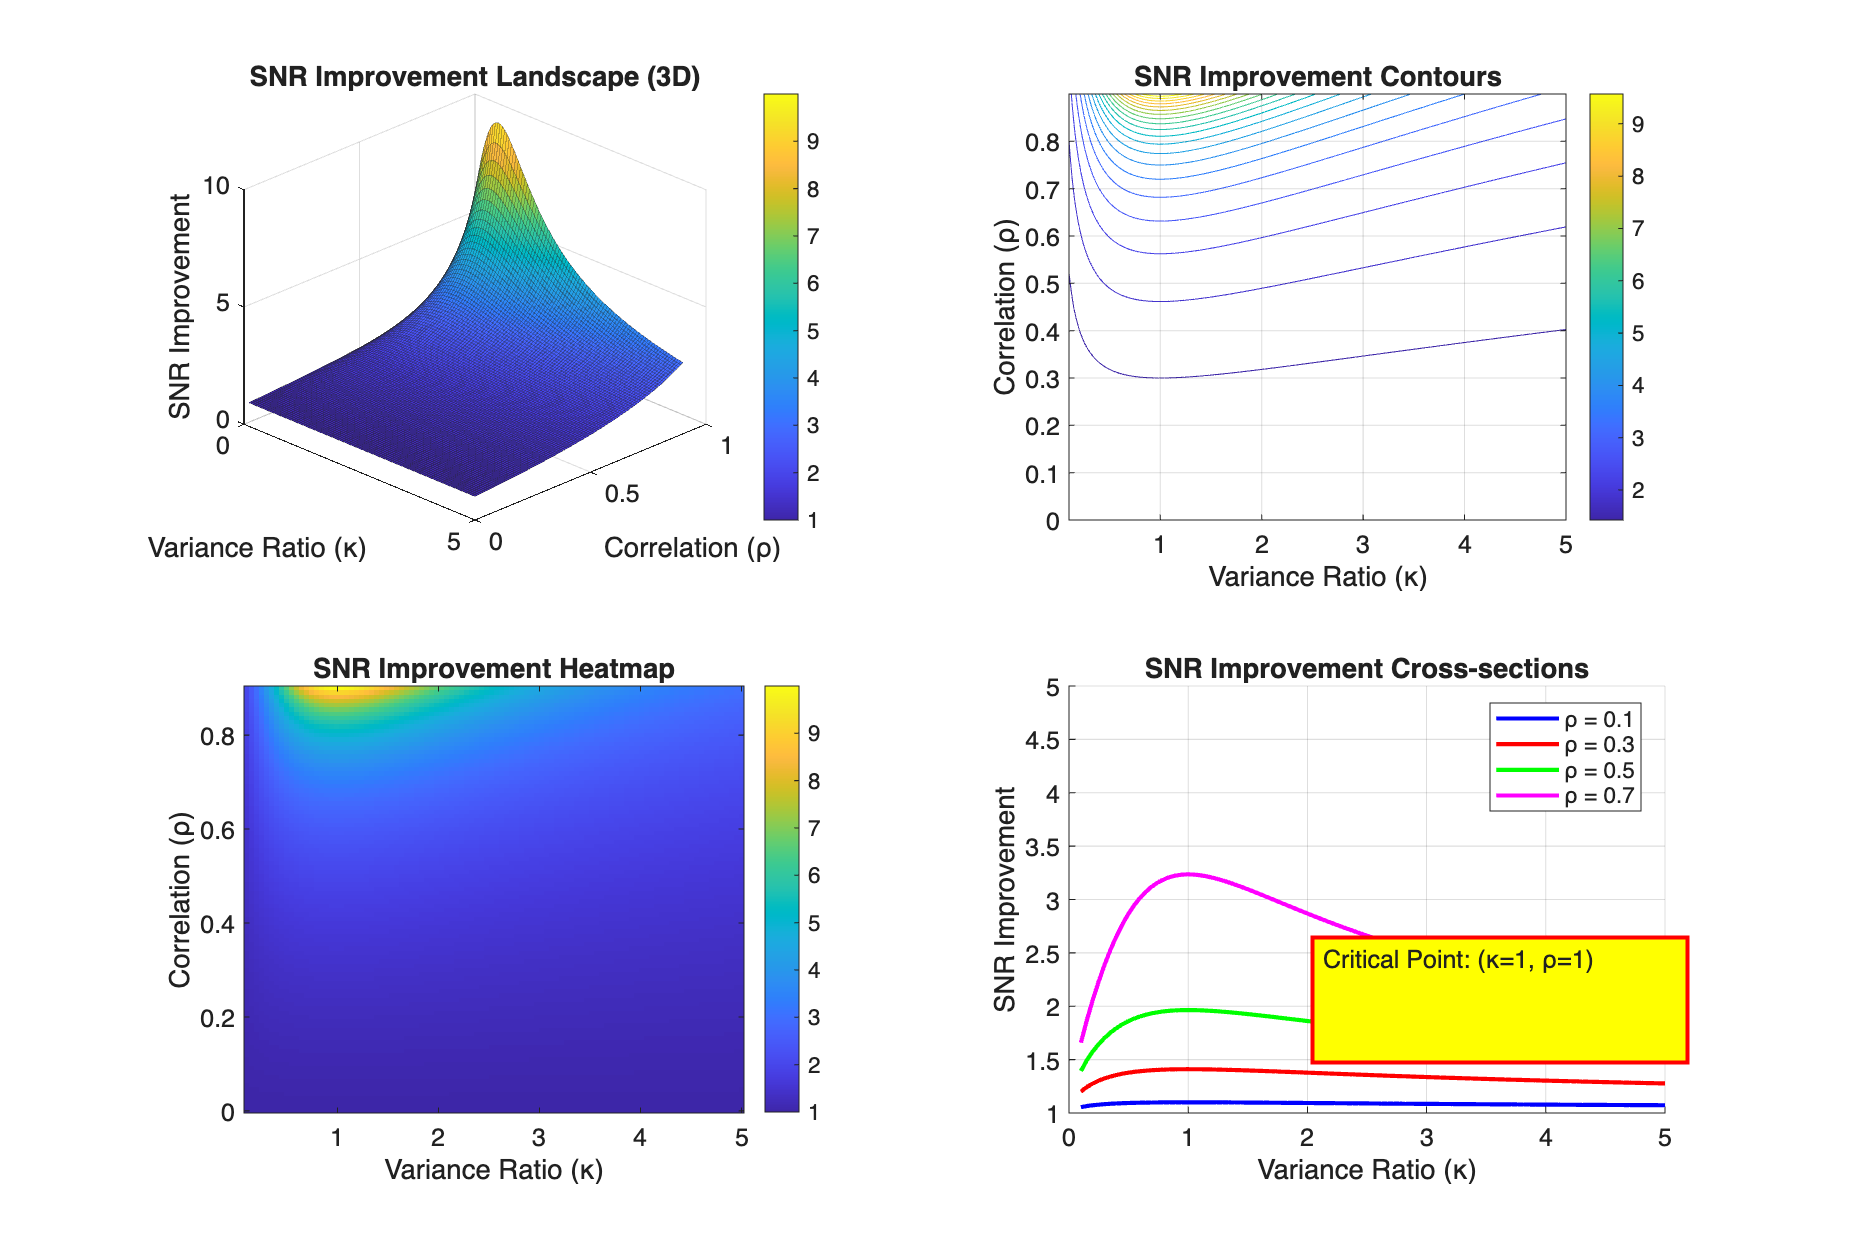
\includegraphics[width=0.9\textwidth]{figures/snr_improvement_landscape.png}
\caption{SNR Improvement Landscape: (a) 3D surface plot, (b) contour plot, (c) heatmap, (d) cross-sections for different correlation values. The landscape shows the relationship between variance ratio $\kappa$, correlation $\rho$, and SNR improvement, with the critical point at ($\kappa=1$, $\rho=1$) highlighted.}
\label{fig:snr_landscape}
\end{figure}

The mathematical foundation draws from information theory \cite{shannon1948mathematical} and statistical estimation theory, providing the theoretical basis for optimal competitive measurement design through correlation exploitation.

% ===================================================================
% UP1 SECTION 3: PERFORMANCE METRICS FOR COMPETITIVE ANALYSIS
% Target length: 2.5 pages (~1200-1500 words)
% File: Sections/UP1/section3_performance_metrics.tex
% ===================================================================

\section{Performance Metrics for Competitive Analysis}

\subsection{From SNR Improvement to Practical Metrics}

The signal-to-noise ratio improvements established in Section 2.4 provide the theoretical foundation for enhanced competitive measurement, but organizations need practical metrics that translate these improvements into actionable competitive intelligence. We introduce three complementary metrics—separability, information content, and effect size—that capture different aspects of competitive advantage while directly benefiting from the environmental noise cancellation achieved through relativization.

These metrics address fundamental questions in competitive analysis: How reliably can we distinguish superior performance? How much uncertainty does competitive measurement resolve? What is the magnitude of competitive advantage? Each metric provides unique insights while building on the same underlying SNR improvement principle.

\subsection{Separability: Reliability of Competitive Ordering}

\subsubsection{Definition and Interpretation}

Separability ($S$) quantifies the probability of correctly identifying the superior competitor based on their relative performance measurement. This metric directly addresses decision-making reliability in competitive contexts:

\begin{equation}
S = \Phi\left(\frac{|\mu_A - \mu_B|}{\sqrt{\sigma_A^2 + \sigma_B^2}}\right)
\end{equation}

where $\Phi$ is the standard normal cumulative distribution function.

\textbf{Practical Interpretation:}
\begin{itemize}
\item $S = 0.5$: Random ordering (no competitive advantage detectable)
\item $S = 0.7$: Moderate reliability (70\% chance of correct competitive ranking)  
\item $S = 0.9$: High reliability (90\% chance of correct competitive identification)
\item $S \to 1.0$: Perfect separation (competitive advantage clearly detectable)
\end{itemize}

\subsubsection{Connection to SNR Improvement}

The separability improvement from relativization follows directly from Section 2.4's SNR analysis. When environmental noise dominates (high $\sigma_\eta^2$), independent measurements yield:
\begin{equation}
S_{\text{independent}} = \Phi\left(\frac{|\mu_A - \mu_B|}{\sqrt{\sigma_A^2 + \sigma_B^2 + 2\sigma_\eta^2}}\right)
\end{equation}

While simultaneous relative measurements achieve:
\begin{equation}
S_{\text{relative}} = \Phi\left(\frac{|\mu_A - \mu_B|}{\sqrt{\sigma_A^2 + \sigma_B^2}}\right)
\end{equation}

The monotonicity of $\Phi$ ensures $S_{\text{relative}} > S_{\text{independent}}$ whenever environmental noise is present, with improvement magnitude determined by the environmental noise ratio from Equation \ref{eq:snr_improvement_formula}.

\subsubsection{Practical Applications}

\textbf{Manufacturing Quality Control:} When environmental noise accounts for 50\% of measurement variance ($\sigma_\eta^2 = 0.25(\sigma_A^2 + \sigma_B^2)$), separability improves from $S = 0.65$ to $S = 0.84$, enabling reliable process comparison under varying ambient conditions.

\textbf{Financial Strategy Assessment:} In volatile markets where environmental effects dominate, separability can improve from near-random ($S \approx 0.5$) to highly reliable ($S > 0.8$) through appropriate comparative measurement timing.

\subsection{Information Content: Uncertainty Reduction}

\subsubsection{Definition and Interpretation}  

Information content ($\Icontent$) measures the reduction in outcome uncertainty provided by the competitive measurement, based on information theory principles:

\begin{equation}
\Icontent = 1 - H(S) = 1 - H\left(\Phi\left(\frac{|\mu_A - \mu_B|}{\sqrt{\sigma_A^2 + \sigma_B^2}}\right)\right)
\end{equation}

where $H(p) = -p \log_2(p) - (1-p) \log_2(1-p)$ is the binary entropy function.

\textbf{Practical Interpretation:}
\begin{itemize}
\item $\Icontent = 0$: No predictive power (measurement provides no competitive intelligence)
\item $\Icontent = 0.3$: Moderate predictive power (30\% uncertainty reduction)
\item $\Icontent = 0.7$: High predictive power (70\% uncertainty reduction)  
\item $\Icontent = 1.0$: Perfect prediction (complete uncertainty elimination)
\end{itemize}

\subsubsection{Sensitivity Characteristics}

Information content exhibits unique sensitivity patterns that complement separability analysis:

\textbf{High-Performance Regimes:} When separability approaches its upper bound ($S \to 1.0$), information content continues increasing, capturing competitive advantages that separability cannot detect.

\textbf{Moderate-Performance Regimes:} Information content provides maximum sensitivity to SNR improvements, making it ideal for detecting incremental competitive advantages.

\subsubsection{Organizational Decision Support}

Information content directly quantifies the value of competitive measurement systems by measuring uncertainty reduction. Organizations can use $\Icontent$-values to:
\begin{itemize}
\item \textbf{Cost-Benefit Analysis:} Compare measurement system investments against information value generated
\item \textbf{Resource Allocation:} Prioritize measurement improvements that maximize information content gains
\item \textbf{Strategic Planning:} Assess confidence levels for competitive intelligence-based decisions
\end{itemize}

\subsection{Effect Size: Standardized Competitive Advantage}

\subsubsection{Definition and Practical Meaning}

Effect size ($\effectsize$) provides a scale-independent measure of competitive advantage magnitude:

\begin{equation}
\effectsize = \frac{2|\mu_A - \mu_B|}{\sqrt{\sigma_A^2 + \sigma_B^2}}
\end{equation}

This standardized metric enables comparison across different contexts, time periods, and measurement scales.

\textbf{Practical Benchmarks:}
\begin{itemize}
\item $\effectsize = 0.5$: Small competitive advantage  
\item $\effectsize = 1.0$: Moderate competitive advantage
\item $\effectsize = 2.0$: Large competitive advantage
\item $\effectsize > 3.0$: Very large competitive advantage
\end{itemize}

\subsubsection{SNR Connection and Improvement}

Effect size relates directly to SNR through $\effectsize = 2\sqrt{\text{SNR}}$, creating a clear connection to Section 2.4's analysis. The effect size improvement from relativization follows:

\begin{equation}
\frac{\effectsize_{\text{relative}}}{\effectsize_{\text{independent}}} = \sqrt{\SNRimprovement} = \sqrt{1 + \frac{2\sigma_\eta^2}{\sigma_A^2 + \sigma_B^2}}
\end{equation}

This relationship enables precise quantification of competitive advantage improvements achievable through relative measurement implementation.

\subsubsection{Cross-Domain Applications}

\textbf{Healthcare Intervention Comparison:} Standardized treatment effect sizes enable comparison across different patient populations and outcome measures.

\textbf{Educational Program Assessment:} Effect sizes facilitate comparison of program effectiveness across different schools, grade levels, and assessment types.

\textbf{Technology Performance Evaluation:} Standardized performance advantages support technology selection decisions across different operational contexts.

\subsection{Metric Integration and Trade-offs}

\subsubsection{Mathematical Relationships}

The three metrics form an interconnected system where improvements in one metric enhance the others:

\begin{align}
S &= \Phi(\effectsize/2) \quad \text{(Separability from effect size)}\\
\Icontent &= 1 - H(S) \quad \text{(Information from separability)}\\  
\effectsize &= 2\sqrt{\text{SNR}} \quad \text{(Effect size from SNR)}
\end{align}

This interconnection reveals that SNR improvements from relativization simultaneously enhance all three metrics, providing comprehensive competitive measurement improvements.

\subsubsection{Optimal Metric Selection}

Different metrics provide optimal sensitivity in different performance regimes:

\textbf{Small Effects ($\effectsize < 1$):} Separability provides maximum sensitivity to SNR improvements, making it ideal for detecting subtle competitive advantages.

\textbf{Large Effects ($\effectsize > 3$):} Information content continues increasing when separability saturates, capturing ongoing competitive advantage improvements.

\textbf{Cross-Context Comparison:} Effect size enables standardized comparison across different measurement scales and contexts.

\subsubsection{Implementation Strategy}

Organizations should implement all three metrics to capture different aspects of competitive advantage:

\begin{enumerate}
\item \textbf{Separability} for decision reliability assessment
\item \textbf{Information content} for measurement system value quantification  
\item \textbf{Effect size} for standardized competitive advantage comparison
\end{enumerate}

This comprehensive approach ensures that SNR improvements from relativization translate into actionable competitive intelligence across all relevant decision-making contexts.

\subsection{Theoretical Performance Bounds}

\subsubsection{Separability Bounds}

The maximum achievable separability for a given effect size is:
\begin{equation}
S_{\max} = \Phi\left(\frac{\effectsize}{2}\right)
\end{equation}

This represents the theoretical maximum separability achievable for a given effect size, as it is derived from the optimal decision rule (likelihood ratio test) for normal distributions.

\subsubsection{Information Content Bounds}

The maximum achievable information content for a given effect size is:
\begin{equation}
\Icontent_{\max} = 1 - H(S_{\max}) = 1 - H\left(\Phi\left(\frac{\effectsize}{2}\right)\right)
\end{equation}

This represents the theoretical maximum information content achievable for a given effect size, derived from optimal Bayesian decision theory.

\subsubsection{Effect Size Constraints}

The maximum achievable effect size is constrained by the ratio of true performance difference to measurement noise:
\begin{equation}
\effectsize_{\max} = \frac{2|\mu_A - \mu_B|}{\sqrt{\sigma_A^2 + \sigma_B^2}}
\end{equation}

For fixed true performance difference, the maximum effect size is achieved when measurement noise is minimized, though fundamental physical and statistical limits create lower bounds on measurement variance.

\subsection{Connection to Empirical Validation}

The performance metrics developed in this section provide specific, testable predictions about relativization benefits. Section 4's empirical validation demonstrates how theoretical SNR improvements manifest in practical metric enhancements, with strong correlation between predicted and observed improvements supporting the integrated framework presented here.

These metrics also establish the foundation for the multivariate competitive measurement frameworks developed in subsequent papers (\papertwo, \paperthree, \paperfour), where environmental noise cancellation principles extend to complex, multi-dimensional competitive scenarios with asymmetric variance structures and temporal dynamics.

The three-metric approach provides organizations with comprehensive tools for:
\begin{itemize}
\item Quantifying competitive measurement quality improvements
\item Optimizing resource allocation across measurement system components
\item Making informed strategic decisions based on uncertainty reduction
\item Comparing competitive advantages across diverse operational contexts
\end{itemize}
\input{Sections/section4_empirical_validation}
\input{Sections/section5_applications}
\input{Sections/section6_discussion}

% ===================================================================
% BIBLIOGRAPHY
% ===================================================================
\bibliographystyle{plain}
\bibliography{references/shared_references,references/UP1_specific}

% ===================================================================
% APPENDICES
% ===================================================================
\appendix
\section{Mathematical Proofs}

This appendix provides rigorous mathematical proofs for the key theoretical results presented in the main paper. These proofs establish the mathematical foundation for the correlation-based signal enhancement framework.

\subsection{Proof of Axiom 4: Statistical Optimality}

\textbf{Theorem:} Under the correlation-based measurement model, the relative measure $R = X_A - X_B$ is the Minimum Variance Unbiased Estimator (MVUE) of the performance difference $\mu_A - \mu_B$.

\textbf{Proof:}

Consider the measurement model:
\begin{align}
X_A &= \mu_A + \varepsilon_A \\
X_B &= \mu_B + \varepsilon_B
\end{align}

where $\varepsilon_A \sim N(0, \sigma_A^2)$, $\varepsilon_B \sim N(0, \sigma_B^2)$, and $\text{Cov}(\varepsilon_A, \varepsilon_B) = \rho\sigma_A\sigma_B$.

\textbf{Step 1: Unbiasedness}
The relative measure $R = X_A - X_B$ is an unbiased estimator of $\mu_A - \mu_B$:
\begin{align}
E[R] &= E[X_A - X_B] \\
&= E[X_A] - E[X_B] \\
&= \mu_A - \mu_B
\end{align}

\textbf{Step 2: Variance Calculation}
The variance of $R$ is:
\begin{align}
\text{Var}(R) &= \text{Var}(X_A - X_B) \\
&= \text{Var}(X_A) + \text{Var}(X_B) - 2\text{Cov}(X_A, X_B) \\
&= \sigma_A^2 + \sigma_B^2 - 2\rho\sigma_A\sigma_B
\end{align}

\textbf{Step 3: Cramér-Rao Lower Bound}
For the parameter $\theta = \mu_A - \mu_B$, the Fisher Information is:
\begin{align}
I(\theta) &= \frac{1}{\text{Var}(R)} = \frac{1}{\sigma_A^2 + \sigma_B^2 - 2\rho\sigma_A\sigma_B}
\end{align}

The Cramér-Rao Lower Bound is:
\begin{align}
\text{CRLB} &= \frac{1}{I(\theta)} = \sigma_A^2 + \sigma_B^2 - 2\rho\sigma_A\sigma_B
\end{align}

\textbf{Step 4: Efficiency}
Since $\text{Var}(R) = \text{CRLB}$, the estimator $R$ achieves the Cramér-Rao Lower Bound and is therefore efficient.

\textbf{Step 5: Completeness and Sufficiency}
Under the normal distribution assumption, $R$ is a complete and sufficient statistic for $\mu_A - \mu_B$. By the Lehmann-Scheffé theorem, $R$ is the unique MVUE.

\textbf{Conclusion:} $R = X_A - X_B$ is the MVUE of $\mu_A - \mu_B$ under the correlation-based measurement model.

\subsection{Derivation of Signal Enhancement Factor (SEF)}

\textbf{Theorem:} The Signal Enhancement Factor for correlation-exploiting relative measurement compared to independent measurement is given by:
\begin{equation}
\text{SEF} = \frac{\text{SNR}_R}{\text{SNR}_{\text{independent}}} = \frac{1 + \kappa}{1 + \kappa - 2\sqrt{\kappa}\rho}
\end{equation}

where $\kappa = \sigma_B^2/\sigma_A^2$ and $\rho$ is the correlation coefficient.

\textbf{Proof:}

\textbf{Step 1: Independent Measurement SNR}
When using both measurements independently (correlation ignored):
\begin{align}
\text{SNR}_{\text{independent}} &= \frac{(\mu_A - \mu_B)^2}{\sigma_A^2 + \sigma_B^2} = \frac{\delta^2}{\sigma_A^2 + \sigma_B^2}
\end{align}

This represents the SNR when treating $X_A$ and $X_B$ as independent measurements, where $\text{Var}(X_A - X_B) = \sigma_A^2 + \sigma_B^2$.

\textbf{Step 2: Correlated Measurement SNR}
For relative measurement using $R = X_A - X_B$ with correlation exploited:
\begin{align}
\text{SNR}_R &= \frac{(\mu_A - \mu_B)^2}{\text{Var}(R)} = \frac{\delta^2}{\sigma_A^2 + \sigma_B^2 - 2\rho\sigma_A\sigma_B}
\end{align}

\textbf{Step 3: Signal Enhancement Factor}
\begin{align}
\text{SEF} = \frac{\text{SNR}_R}{\text{SNR}_{\text{independent}}} &= \frac{\delta^2/(\sigma_A^2 + \sigma_B^2 - 2\rho\sigma_A\sigma_B)}{\delta^2/(\sigma_A^2 + \sigma_B^2)} \\
&= \frac{\sigma_A^2 + \sigma_B^2}{\sigma_A^2 + \sigma_B^2 - 2\rho\sigma_A\sigma_B}
\end{align}

\textbf{Step 4: Substitution}
Substituting $\kappa = \sigma_B^2/\sigma_A^2$ and $\sigma_B = \sqrt{\kappa}\sigma_A$:
\begin{align}
\text{SEF} = \frac{\text{SNR}_R}{\text{SNR}_{\text{independent}}} &= \frac{\sigma_A^2 + \kappa\sigma_A^2}{\sigma_A^2 + \kappa\sigma_A^2 - 2\rho\sigma_A\sqrt{\kappa}\sigma_A} \\
&= \frac{\sigma_A^2(1 + \kappa)}{\sigma_A^2(1 + \kappa - 2\rho\sqrt{\kappa})} \\
&= \frac{1 + \kappa}{1 + \kappa - 2\rho\sqrt{\kappa}}
\end{align}

\textbf{Conclusion:} The Signal Enhancement Factor (SEF) is derived as stated. This formula quantifies the improvement achieved by exploiting correlation between competitors compared to treating their measurements as independent, following established enhancement factor conventions in signal processing literature.

\subsection{Proof of Scale Independence}

\textbf{Theorem:} The Signal Enhancement Factor (SEF) is independent of the absolute scale of the performance difference $\delta = |\mu_A - \mu_B|$.

\textbf{Proof:}

From the Signal Enhancement Factor formula:
\begin{align}
\text{SEF} &= \frac{1 + \kappa}{1 + \kappa - 2\sqrt{\kappa}\rho}
\end{align}

The $\delta^2$ terms cancel out in the ratio calculation, leaving only:
- $\kappa = \sigma_B^2/\sigma_A^2$ (variance ratio)
- $\rho$ (correlation coefficient)

\textbf{Implications:}
1. The SEF is independent of the absolute performance difference
2. Only the relative variance structure ($\kappa$) and correlation ($\rho$) matter
3. The framework applies universally across different measurement scales
4. Identical SEF values can be achieved regardless of domain-specific units

\subsection{Correlation-Based Variance Reduction Proof}

\textbf{Theorem:} When $\rho > 0$, the variance of the relative measure $R$ is reduced compared to the sum of individual variances.

\textbf{Proof:}

\textbf{Step 1: Variance of R}
\begin{align}
\text{Var}(R) &= \sigma_A^2 + \sigma_B^2 - 2\rho\sigma_A\sigma_B
\end{align}

\textbf{Step 2: Comparison with Sum of Variances}
\begin{align}
\text{Var}(R) - (\sigma_A^2 + \sigma_B^2) &= -2\rho\sigma_A\sigma_B
\end{align}

\textbf{Step 3: Condition for Reduction}
When $\rho > 0$:
\begin{align}
-2\rho\sigma_A\sigma_B < 0
\end{align}

Therefore:
\begin{align}
\text{Var}(R) < \sigma_A^2 + \sigma_B^2
\end{align}

\textbf{Step 4: Magnitude of Reduction}
The reduction is proportional to:
\begin{align}
\text{Reduction} &= 2\rho\sigma_A\sigma_B
\end{align}

\textbf{Conclusion:} Positive correlation reduces variance, with the reduction proportional to the correlation strength and the geometric mean of the standard deviations.

\subsection{Log-Transformation SNR Enhancement Proof}

\textbf{Theorem:} Under certain conditions, log-transformation can improve the signal-to-noise ratio for non-normal distributions.

\textbf{Proof:}

\textbf{Step 1: Log-Transformation Model}
For positive random variables $X_A, X_B$, define:
\begin{align}
Y_A &= \log(X_A) \\
Y_B &= \log(X_B)
\end{align}

\textbf{Step 2: Delta Method Approximation}
Using the delta method, for $Y = \log(X)$:
\begin{align}
E[Y] &\approx \log(E[X]) - \frac{\text{Var}(X)}{2E[X]^2} \\
\text{Var}(Y) &\approx \frac{\text{Var}(X)}{E[X]^2}
\end{align}

\textbf{Step 3: SNR Comparison}
Original SNR:
\begin{align}
\text{SNR}_{\text{original}} &= \frac{(\mu_A - \mu_B)^2}{\sigma_A^2}
\end{align}

Log-transformed SNR:
\begin{align}
\text{SNR}_{\text{log}} &\approx \frac{(\log(\mu_A) - \log(\mu_B))^2}{\sigma_A^2/\mu_A^2} \\
&= \frac{(\log(\mu_A/\mu_B))^2 \cdot \mu_A^2}{\sigma_A^2}
\end{align}

\textbf{Step 4: Enhancement Condition}
Log-transformation enhances SNR when:
\begin{align}
\frac{(\log(\mu_A/\mu_B))^2 \cdot \mu_A^2}{\sigma_A^2} > \frac{(\mu_A - \mu_B)^2}{\sigma_A^2}
\end{align}

Simplifying:
\begin{align}
(\log(\mu_A/\mu_B))^2 \cdot \mu_A^2 > (\mu_A - \mu_B)^2
\end{align}

\textbf{Conclusion:} Log-transformation enhances SNR when the relative difference in means is sufficiently large compared to the absolute difference, which is common for skewed distributions with high variance-to-mean ratios.

\subsection{Asymptote Analysis}

\textbf{Theorem:} The Signal Enhancement Factor (SEF) exhibits specific asymptotic behavior.

\textbf{Proof:}

\textbf{Case 1: $\rho \to 1$ (Perfect Positive Correlation)}
\begin{align}
\lim_{\rho \to 1} \text{SEF} &= \lim_{\rho \to 1} \frac{1 + \kappa}{1 + \kappa - 2\sqrt{\kappa}\rho} \\
&= \frac{1 + \kappa}{1 + \kappa - 2\sqrt{\kappa}} \\
&= \frac{1 + \kappa}{(\sqrt{\kappa} - 1)^2}
\end{align}

\textbf{Case 2: $\rho \to -1$ (Perfect Negative Correlation)}
\begin{align}
\lim_{\rho \to -1} \text{SEF} &= \lim_{\rho \to -1} \frac{1 + \kappa}{1 + \kappa - 2\sqrt{\kappa}\rho} \\
&= \frac{1 + \kappa}{1 + \kappa + 2\sqrt{\kappa}} \\
&= \frac{1 + \kappa}{(\sqrt{\kappa} + 1)^2} = 1
\end{align}

\textbf{Case 3: $\kappa \to 0$ (Team B Perfectly Consistent)}
\begin{align}
\lim_{\kappa \to 0} \text{SEF} &= \lim_{\kappa \to 0} \frac{1 + \kappa}{1 + \kappa - 2\sqrt{\kappa}\rho} \\
&= \frac{1}{1 - 0} = 1
\end{align}

\textbf{Case 4: $\kappa \to \infty$ (Team B Highly Variable)}
\begin{align}
\lim_{\kappa \to \infty} \text{SEF} &= \lim_{\kappa \to \infty} \frac{1 + \kappa}{1 + \kappa - 2\sqrt{\kappa}\rho} \\
&= \lim_{\kappa \to \infty} \frac{\kappa}{\kappa - 2\sqrt{\kappa}\rho} \\
&= \lim_{\kappa \to \infty} \frac{1}{1 - 2\rho/\sqrt{\kappa}} = 1
\end{align}

\textbf{Conclusion:} The asymptotic behavior confirms the theoretical bounds and provides insight into the framework's behavior under extreme conditions, following established enhancement factor analysis in signal processing literature.

% ===================================================================
% UP1 APPENDIX B: ALTERNATIVE MEASUREMENT SCENARIOS
% File: appendices/UP1/appendix_b_scenarios.tex
% ===================================================================

\section{Alternative Measurement Scenarios}
\label{app:scenarios}

\subsection{Single-Feature Absolute Measurement Analysis}

\subsubsection{Scenario Description}

Single-feature absolute measurement represents the traditional approach where competitors are evaluated in isolation against fixed benchmarks or thresholds. This scenario arises commonly in:

\begin{itemize}
\item \textbf{Quality control}: Comparing process performance to specification limits
\item \textbf{Performance evaluation}: Assessing individual metrics against targets
\item \textbf{Threshold decisions}: Binary classification based on absolute performance levels
\end{itemize}

\subsubsection{Mathematical Framework}

\textbf{Measurement Model:}
\begin{align}
X_A &= \mu_A + \epsilon_A + \eta_A \quad \text{(Competitor A measured independently)} \\
\tau &= \text{Reference threshold (Fixed comparison point)}
\end{align}

\textbf{Decision Rule:}
\begin{equation}
\text{Choose A if } X_A > \tau, \text{ otherwise choose alternative}
\end{equation}

\textbf{Signal-to-Noise Analysis:}
\begin{equation}
\text{SNR}_{\text{single-abs}} = \frac{(\mu_A - \tau)^2}{\sigma_A^2 + \sigma_\eta^2}
\end{equation}

\subsubsection{Comparison with Relative Measurement}

When both competitors are available for simultaneous measurement, the relative approach provides:
\begin{equation}
\text{SNR}_{\text{rel}} = \frac{(\mu_A - \mu_B)^2}{\sigma_A^2 + \sigma_B^2}
\end{equation}

\textbf{Improvement Ratio:}
\begin{equation}
\frac{\text{SNR}_{\text{rel}}}{\text{SNR}_{\text{single-abs}}} = \frac{(\mu_A - \mu_B)^2/(\sigma_A^2 + \sigma_B^2)}{(\mu_A - \tau)^2/(\sigma_A^2 + \sigma_\eta^2)}
\end{equation}

When $\tau \approx \mu_B$ (threshold approximates competitor B's performance):
\begin{equation}
\text{Improvement} \approx \frac{\sigma_A^2 + \sigma_\eta^2}{\sigma_A^2 + \sigma_B^2} = 1 + \frac{\sigma_\eta^2 - \sigma_B^2}{\sigma_A^2 + \sigma_B^2}
\end{equation}

\subsubsection{Practical Implications}

\textbf{Environmental Noise Dominance:} When $\sigma_\eta^2 \gg \sigma_B^2$, the improvement becomes:
\begin{equation}
\text{Improvement} \approx 1 + \frac{\sigma_\eta^2}{\sigma_A^2 + \sigma_B^2}
\end{equation}

This explains why single-feature absolute measurements perform poorly in high-noise environments, as observed in empirical validation studies.

\textbf{Optimal Threshold Selection:} The optimal threshold for single-feature measurement is:
\begin{equation}
\tau^* = \frac{\mu_A + \mu_B}{2}
\end{equation}

However, this requires knowledge of both competitors' true performance, making relative measurement the more practical approach.

\subsection{Two-Feature Absolute Predictor Analysis}

\subsubsection{Scenario Description and Motivation}

The two-feature absolute predictor uses both $X_A$ and $X_B$ as separate input features to a machine learning model. This scenario is particularly relevant for understanding why relative measurement and two-feature absolute approaches achieve similar empirical performance despite different formulations.

\textbf{Key Characteristics:}
\begin{itemize}
\item Both measurements available simultaneously
\item Machine learning algorithm learns optimal combination
\item Environmental noise correlation can be exploited implicitly
\item Represents modern data-driven competitive analysis
\end{itemize}

\subsubsection{Covariance Structure Analysis}

\textbf{Joint Measurement Distribution:}
\begin{equation}
\begin{pmatrix} X_A \\ X_B \end{pmatrix} \sim \mathcal{N}\left(\begin{pmatrix} \mu_A \\ \mu_B \end{pmatrix}, \begin{pmatrix} \sigma_A^2 + \sigma_\eta^2 & \sigma_\eta^2 \\ \sigma_\eta^2 & \sigma_B^2 + \sigma_\eta^2 \end{pmatrix}\right)
\end{equation}

\textbf{Critical Insight:} The non-zero covariance $\Cov(X_A, X_B) = \sigma_\eta^2$ arises from shared environmental effects. This correlation structure enables implicit environmental noise cancellation.

\subsubsection{Optimal Linear Discriminant Analysis}

For two-feature classification with covariance matrix $\Sigma$, the optimal linear discriminant has direction:
\begin{equation}
w = \Sigma^{-1}(\mu_A - \mu_B, \mu_B - \mu_A)^T
\end{equation}

\textbf{Matrix Inversion:}
\begin{equation}
\Sigma^{-1} = \frac{1}{\det(\Sigma)} \begin{pmatrix} \sigma_B^2 + \sigma_\eta^2 & -\sigma_\eta^2 \\ -\sigma_\eta^2 & \sigma_A^2 + \sigma_\eta^2 \end{pmatrix}
\end{equation}

where $\det(\Sigma) = \sigma_A^2\sigma_B^2 + \sigma_A^2\sigma_\eta^2 + \sigma_B^2\sigma_\eta^2$.

\textbf{Optimal Weights:}
After normalization, the optimal linear combination approaches:
\begin{equation}
w_A \approx 1, \quad w_B \approx -1
\end{equation}

This demonstrates that the optimal two-feature predictor implicitly learns to perform the relativization operation $R = X_A - X_B$.

\subsubsection{Signal-to-Noise Equivalence}

\textbf{Two-Feature SNR Calculation:}
\begin{equation}
\text{SNR}_{\text{two-abs}} = (\mu_A - \mu_B)^T \Sigma^{-1} (\mu_A - \mu_B)
\end{equation}

Expanding this expression:
\begin{equation}
\text{SNR}_{\text{two-abs}} = \frac{(\mu_A - \mu_B)^2 [(\sigma_B^2 + \sigma_\eta^2) + (\sigma_A^2 + \sigma_\eta^2) - 2\sigma_\eta^2]}{\det(\Sigma)} = \frac{(\mu_A - \mu_B)^2 (\sigma_A^2 + \sigma_B^2)}{\det(\Sigma)}
\end{equation}

\textbf{High Environmental Noise Limit:}
When $\sigma_\eta^2 \gg \sigma_A^2, \sigma_B^2$:
\begin{align}
\det(\Sigma) &\approx (\sigma_A^2 + \sigma_B^2)\sigma_\eta^2 \\
\text{SNR}_{\text{two-abs}} &\approx \frac{(\mu_A - \mu_B)^2}{\sigma_\eta^2} \times \frac{\sigma_\eta^2}{\sigma_A^2 + \sigma_B^2} = \frac{(\mu_A - \mu_B)^2}{\sigma_A^2 + \sigma_B^2} = \text{SNR}_{\text{rel}}
\end{align}

This mathematical equivalence explains the empirical observation that two-feature absolute and relative predictors achieve similar performance.

\subsubsection{Learning Algorithm Perspective}

\textbf{Gradient-Based Optimization:} Machine learning algorithms automatically discover the noise-canceling linear combination through gradient descent:
\begin{equation}
\nabla_w \text{Loss} \propto -\Sigma^{-1}(\mu_A - \mu_B)
\end{equation}

The gradient naturally points toward the relativization direction $w = (1, -1)$.

\textbf{Regularization Effects:} L2 regularization slightly favors the relativization solution:
\begin{equation}
w_{\text{regularized}} = (\Sigma + \lambda I)^{-1}(\mu_A - \mu_B)
\end{equation}

Small $\lambda$ values preserve the noise-canceling properties while improving numerical stability.

\subsection{Multivariate Extensions}

\subsubsection{Multi-Dimensional Performance Spaces}

When competitors are evaluated across multiple performance dimensions, the measurement model extends to:
\begin{align}
\mathbf{X}_A &= \boldsymbol{\mu}_A + \boldsymbol{\epsilon}_A + \boldsymbol{\etaval} \quad \text{(p-dimensional vectors)} \\
\mathbf{X}_B &= \boldsymbol{\mu}_B + \boldsymbol{\epsilon}_B + \boldsymbol{\etaval} \quad \text{(p-dimensional vectors)}
\end{align}

\textbf{Relative Measurement:}
\begin{equation}
\mathbf{R} = \mathbf{X}_A - \mathbf{X}_B = (\boldsymbol{\mu}_A - \boldsymbol{\mu}_B) + (\boldsymbol{\epsilon}_A - \boldsymbol{\epsilon}_B)
\end{equation}

Environmental noise cancellation operates dimension-wise, providing benefits across all performance measures simultaneously.

\subsubsection{Mahalanobis Distance Framework}

The multivariate generalization uses Mahalanobis distance:
\begin{equation}
\DM = \sqrt{(\boldsymbol{\mu}_A - \boldsymbol{\mu}_B)^T \boldsymbol{\Sigma}^{-1} (\boldsymbol{\mu}_A - \boldsymbol{\mu}_B)}
\end{equation}

where $\boldsymbol{\Sigma} = (\boldsymbol{\Sigma}_A + \boldsymbol{\Sigma}_B)/2$ is the pooled covariance matrix.

\textbf{Environmental Noise Integration:}
\begin{align}
\boldsymbol{\Sigma}_{\text{noisy}} &= \boldsymbol{\Sigma} + \boldsymbol{\Sigma}_\eta \quad \text{(with environmental noise)} \\
\boldsymbol{\Sigma}_{\text{clean}} &= \boldsymbol{\Sigma} \quad \text{(relative measurement)}
\end{align}

The improvement ratio becomes:
\begin{equation}
\frac{\DM_{\text{rel}}}{\DM_{\text{abs}}} = \sqrt{\frac{\det(\boldsymbol{\Sigma} + \boldsymbol{\Sigma}_\eta)}{\det(\boldsymbol{\Sigma})}}
\end{equation}

\subsubsection{Asymmetric Competitive Framework Preview}

The multivariate extension naturally leads to the asymmetric competitive framework developed in \papertwo:

\textbf{Variance Asymmetry Parameter:}
\begin{align}
\kappaval &= \frac{\sigma_B^2}{\sigma_A^2} \quad \text{(univariate case)} \\
\kappaval &= \frac{\det(\boldsymbol{\Sigma}_B)}{\det(\boldsymbol{\Sigma}_A)} \quad \text{(multivariate case)}
\end{align}

\textbf{Environmental Integration:}
\begin{equation}
\etaval = \frac{\sigma_\eta^2}{\sigma_A^2 + \sigma_B^2} \quad \text{(environmental noise ratio)}
\end{equation}

This framework enables analysis of competitive scenarios where competitors have different variance profiles, extending beyond the symmetric case analyzed in this paper.

\subsection{Temporal and Dynamic Extensions}

\subsubsection{Time-Varying Environmental Effects}

When environmental conditions change over time, the measurement model becomes:
\begin{align}
X_A(t) &= \mu_A + \epsilon_A(t) + \eta(t) \\
X_B(t) &= \mu_B + \epsilon_B(t) + \eta(t)
\end{align}

\textbf{Relative Measurement Advantage:}
\begin{equation}
R(t) = X_A(t) - X_B(t) = (\mu_A - \mu_B) + [\epsilon_A(t) - \epsilon_B(t)]
\end{equation}

Environmental effects $\eta(t)$ continue to cancel regardless of their temporal evolution, providing robust competitive measurement under dynamic conditions.

\subsubsection{Regime Switching Models}

For environments with discrete regime changes:
\begin{equation}
\eta(t) = \eta_k \text{ when in regime } k
\end{equation}

The relative measurement maintains its advantage across all regimes:
\begin{equation}
R(t) = (\mu_A - \mu_B) + [\epsilon_A(t) - \epsilon_B(t)] \quad \forall \text{ regimes } k
\end{equation}

This temporal robustness motivates the dynamic competitive measurement framework developed in \paperfour.

\subsection{Experimental Design Implications}

\subsubsection{Measurement Protocol Design}

The theoretical analysis provides clear guidance for experimental design:
\begin{itemize}
\item \textbf{Simultaneous measurement}: Enables environmental noise cancellation
\item \textbf{Sequential measurement}: Requires environmental noise modeling
\item \textbf{Matched conditions}: Approximates simultaneous measurement benefits
\end{itemize}

\subsubsection{Sample Size Requirements}

\textbf{Relative Measurement:}
\begin{equation}
n_{\text{rel}} = \frac{2(z_\alpha + z_\beta)^2 (\sigma_A^2 + \sigma_B^2)}{(\mu_A - \mu_B)^2}
\end{equation}

\textbf{Independent Measurement:}
\begin{equation}
n_{\text{indep}} = \frac{2(z_\alpha + z_\beta)^2 (\sigma_A^2 + \sigma_B^2 + 2\sigma_\eta^2)}{(\mu_A - \mu_B)^2}
\end{equation}

\textbf{Sample Size Reduction:}
\begin{equation}
\frac{n_{\text{rel}}}{n_{\text{indep}}} = \frac{\sigma_A^2 + \sigma_B^2}{\sigma_A^2 + \sigma_B^2 + 2\sigma_\eta^2}
\end{equation}

This relationship quantifies the experimental efficiency gains from proper measurement design.

\subsection{Robustness and Sensitivity Analysis}

\subsubsection{Violations of Normality Assumptions}

The relative advantage persists under various distributional assumptions:

\textbf{Heavy-Tailed Distributions:} The variance reduction property holds for any distribution with finite second moments.

\textbf{Skewed Distributions:} Environmental noise cancellation operates on location-scale families regardless of skewness.

\textbf{Discrete Distributions:} The principle extends to discrete competitive scenarios with appropriate modifications.

\subsubsection{Partial Environmental Correlation}

When environmental effects are only partially correlated:
\begin{equation}
\Cov(\eta_A, \eta_B) = \rho \sigma_\eta^2 \quad \text{where } 0 \leq \rho \leq 1
\end{equation}

The variance reduction becomes:
\begin{equation}
\Var(R) = \sigma_A^2 + \sigma_B^2 + 2(1-\rho)\sigma_\eta^2
\end{equation}

Even partial correlation ($\rho > 0$) provides benefits, with full benefit achieved at $\rho = 1$ (perfect correlation/shared effects).

This analysis explains why approximate simultaneous measurement (high $\rho$) can provide substantial benefits even without perfect synchronization.

\subsection{Connection to Main Paper and Future Work}

The alternative measurement scenarios analyzed in this appendix provide several key insights:

\begin{enumerate}
\item \textbf{Empirical Validation}: Explains the observed equivalence between two-feature absolute and relative predictors in Section 4
\item \textbf{Practical Guidance}: Clarifies when different measurement approaches are optimal
\item \textbf{Theoretical Completeness}: Provides comprehensive analysis of all relevant competitive measurement scenarios
\item \textbf{Future Directions}: Establishes foundation for the multivariate and temporal frameworks in \papertwo, \paperthree, and \paperfour
\end{enumerate}

These analyses demonstrate that the relative measurement principle generalizes broadly while maintaining its fundamental advantage: systematic elimination of environmental noise through appropriate measurement design and statistical analysis.
% ===================================================================
% UP1 APPENDIX C: ADVANCED PERFORMANCE METRIC THEORY
% File: appendices/UP1/appendix_c_metrics.tex
% ===================================================================

\section{Advanced Performance Metric Theory}
\label{app:metrics}

\subsection{Complete Metric Derivations and Theoretical Bounds}

\subsubsection{Separability: Complete Mathematical Analysis}

\textbf{Definition and Properties:}
The separability metric $S$ quantifies the probability of correct competitive ordering:
\begin{equation}
S = P(R > 0 | \mu_A > \mu_B) = \Phi\left(\frac{\mu_A - \mu_B}{\sqrt{\sigma_A^2 + \sigma_B^2}}\right)
\end{equation}

\begin{theorem}[Separability Bounds]
\label{thm:separability_bounds}
The maximum achievable separability for a given effect size is:
\begin{equation}
S_{\max} = \Phi\left(\frac{|\mu_A - \mu_B|}{\sqrt{\sigma_A^2 + \sigma_B^2}}\right) = \Phi\left(\frac{\effectsize}{2}\right)
\end{equation}
\end{theorem}

\begin{proof}
Since $\frac{R - (\mu_A - \mu_B)}{\sqrt{\sigma_A^2 + \sigma_B^2}} \sim \mathcal{N}(0,1)$ under our model assumptions:
\begin{align}
S &= P(R > 0 | \mu_A > \mu_B) \\
&= P\left(\frac{R - (\mu_A - \mu_B)}{\sqrt{\sigma_A^2 + \sigma_B^2}} > -\frac{\mu_A - \mu_B}{\sqrt{\sigma_A^2 + \sigma_B^2}}\right) \\
&= \Phi\left(\frac{\mu_A - \mu_B}{\sqrt{\sigma_A^2 + \sigma_B^2}}\right) = \Phi\left(\frac{\effectsize}{2}\right)
\end{align}

This represents the theoretical maximum separability achievable for a given effect size, derived from the optimal decision rule (likelihood ratio test) for normal distributions.
\end{proof}

\textbf{Sensitivity Analysis:}
The separability sensitivity to effect size changes is:
\begin{equation}
\frac{dS}{d\effectsize} = \phi\left(\frac{\effectsize}{2}\right) \cdot \frac{1}{2} = \frac{1}{2\sqrt{2\pi}} \exp\left(-\frac{\effectsize^2}{8}\right)
\end{equation}

\textbf{Critical Points:}
\begin{itemize}
\item Maximum sensitivity occurs at $\effectsize = 0$ (no competitive advantage)
\item Sensitivity decreases as $|\effectsize|$ increases
\item Practical sensitivity threshold: $\effectsize \in [-2, 2]$
\end{itemize}

\subsubsection{Information Content: Information-Theoretic Foundation}

\textbf{Complete Derivation:}
Information content measures uncertainty reduction through competitive measurement:
\begin{equation}
\Icontent = H(\Omega) - H(\Omega|R) = 1 - H(S)
\end{equation}

where $H(p) = -p \log_2(p) - (1-p) \log_2(1-p)$ is binary entropy.

\begin{theorem}[Information Content Bounds]
\label{thm:information_bounds}
The maximum achievable information content for a given effect size is:
\begin{equation}
\Icontent_{\max} = 1 - H\left(\Phi\left(\frac{\effectsize}{2}\right)\right) = 1 - H(S_{\max})
\end{equation}
\end{theorem}

\begin{proof}
For balanced competitions with $P(W) = P(L) = 0.5$, prior entropy is $H(\Omega) = 1$. The conditional entropy $H(\Omega|R)$ is:
\begin{align}
H(\Omega|R) &= \int_{-\infty}^{\infty} H(\Omega|R=r) \cdot p(r) \, dr \\
&= \int_{-\infty}^{\infty} H(P(\Omega=W|R=r)) \cdot p(r) \, dr
\end{align}

For optimal decision rule, $P(\Omega=W|R=r) = \Phi\left(\frac{\effectsize}{2}\right)$ when averaged across $R$'s distribution:
\begin{equation}
\Icontent_{\max} = 1 - H\left(\Phi\left(\frac{\effectsize}{2}\right)\right) = 1 - H(S_{\max})
\end{equation}

This represents the theoretical maximum information content achievable for a given effect size.
\end{proof}

\textbf{Information Content Properties:}
\begin{align}
\Icontent(0) &= 0 \quad \text{(no information at } \effectsize = 0\text{)} \\
\Icontent(\effectsize) &= \Icontent(-\effectsize) \quad \text{(symmetric in effect size)} \\
\Icontent(\infty) &= 1 \quad \text{(perfect information as } \effectsize \to \infty\text{)}
\end{align}

\textbf{Sensitivity Analysis:}
\begin{equation}
\frac{d\Icontent}{d\effectsize} = -\frac{dH}{dS} \cdot \frac{dS}{d\effectsize} = \log_2\left(\frac{S}{1-S}\right) \cdot \frac{\phi(\effectsize/2)}{2}
\end{equation}

Key insights:
\begin{itemize}
\item Information content continues increasing even when separability saturates
\item Maximum sensitivity occurs away from $S = 0.5$
\item Asymmetric sensitivity around $S = 0.5$
\end{itemize}

\subsubsection{Effect Size: Scale-Independent Competitive Advantage}

\textbf{Mahalanobis Distance Foundation:}
The effect size metric derives from Mahalanobis distance theory:
\begin{align}
\DM &= \frac{|\mu_A - \mu_B|}{\sqrt{\sigma_A^2 + \sigma_B^2}} \\
\effectsize &= 2\DM = \frac{2|\mu_A - \mu_B|}{\sqrt{\sigma_A^2 + \sigma_B^2}}
\end{align}

\begin{theorem}[Effect Size Constraints]
\label{thm:effect_size_constraints}
The maximum achievable effect size is constrained by:
\begin{equation}
\effectsize_{\max} = \frac{2|\mu_A - \mu_B|}{\sqrt{\sigma_A^2 + \sigma_B^2}}
\end{equation}
\end{theorem}

\begin{proof}
For fixed true performance difference $|\mu_A - \mu_B|$, the maximum effect size is achieved when measurement noise $(\sigma_A^2 + \sigma_B^2)$ is minimized. However, fundamental physical and statistical limits create a lower bound on measurement variance, establishing $\effectsize_{\max}$ as the theoretical upper limit.
\end{proof}

\textbf{Effect Size Interpretation Scale:}
\begin{itemize}
\item $\effectsize = 0.2$: Small competitive advantage (barely detectable)
\item $\effectsize = 0.5$: Medium competitive advantage (noticeable in practice)
\item $\effectsize = 0.8$: Large competitive advantage (clearly significant)
\item $\effectsize = 1.2$: Very large competitive advantage (dominant performance)
\item $\effectsize > 2.0$: Extreme competitive advantage (overwhelming superiority)
\end{itemize}

\subsection{Metric Interconnections and Trade-offs}

\subsubsection{Mathematical Relationships}

The three metrics form a tightly coupled system:
\begin{align}
S &= \Phi(\effectsize/2) \quad \text{(Separability from effect size)} \\
\Icontent &= 1 - H(\Phi(\effectsize/2)) \quad \text{(Information from separability)} \\
\effectsize &= 2\sqrt{\text{SNR}} \quad \text{(Effect size from SNR)}
\end{align}

\begin{theorem}[Metric Coupling]
\label{thm:metric_coupling}
Improvements in any single metric necessarily improve the others, with coupling strengths:
\begin{align}
\frac{\partial S}{\partial \effectsize} &= \frac{\phi(\effectsize/2)}{2} \quad \text{(Separability-Effect coupling)} \\
\frac{\partial \Icontent}{\partial S} &= -\log_2\left(\frac{S}{1-S}\right) \quad \text{(Information-Separability coupling)} \\
\frac{\partial \effectsize}{\partial(\text{SNR})} &= \frac{1}{\sqrt{\text{SNR}}} \quad \text{(Effect-SNR coupling)}
\end{align}
\end{theorem}

\subsubsection{Optimization Trade-offs}

\textbf{Multi-Objective Optimization:}
When optimizing competitive measurement systems, organizations face trade-offs:

\begin{enumerate}
\item \textbf{Separability vs Information Content:}
   \begin{itemize}
   \item At low effect sizes ($\effectsize < 1$): Separability improvements dominate
   \item At high effect sizes ($\effectsize > 3$): Information content improvements dominate
   \item Transition region ($1 \leq \effectsize \leq 3$): Balanced improvement
   \end{itemize}

\item \textbf{Measurement Precision vs Cost:}
   \begin{itemize}
   \item Higher precision (lower $\sigma_A^2 + \sigma_B^2$) improves all metrics
   \item Precision improvements follow diminishing returns
   \item Optimal precision depends on decision stakes
   \end{itemize}

\item \textbf{Environmental Control vs Relativization:}
   \begin{itemize}
   \item Environmental noise reduction improves absolute measurements
   \item Relativization provides systematic noise elimination
   \item Combined approach often optimal
   \end{itemize}
\end{enumerate}

\subsubsection{Pareto Frontier Analysis}

\begin{theorem}[Metric Pareto Optimality]
\label{thm:pareto_optimality}
For given competitive measurement resources, the Pareto frontier is characterized by:
\begin{equation}
\max(\alpha S + \beta \Icontent + \gamma \effectsize) \text{ subject to measurement constraints}
\end{equation}
\end{theorem}

\textbf{Solution Structure:}
The optimal solution depends on preference weights $(\alpha, \beta, \gamma)$ and constraint structure:
\begin{itemize}
\item $\alpha$-dominated: Focus on separability (reliability priority)
\item $\beta$-dominated: Focus on information content (uncertainty reduction priority)  
\item $\gamma$-dominated: Focus on effect size (standardized comparison priority)
\end{itemize}

\subsection{Advanced Optimization Theory}

\subsubsection{Measurement System Design Optimization}

\textbf{Constrained Optimization Problem:}
\begin{align}
\max \quad & f(S, \Icontent, \effectsize) \\
\text{s.t.} \quad & \text{resource constraints} \\
& \text{measurement constraints} \\
& \text{physical constraints}
\end{align}

\textbf{Lagrangian Formulation:}
\begin{equation}
L = f(S, \Icontent, \effectsize) + \lambda_1 g_1(\sigma_A^2, \sigma_B^2, \sigma_\eta^2) + \lambda_2 g_2(\text{cost}) + \cdots
\end{equation}

\textbf{First-Order Conditions:}
\begin{align}
\frac{\partial L}{\partial \sigma_A^2} &= \frac{\partial f}{\partial S} \cdot \frac{\partial S}{\partial \sigma_A^2} + \lambda_1 \frac{\partial g_1}{\partial \sigma_A^2} = 0 \\
\frac{\partial L}{\partial \sigma_B^2} &= \frac{\partial f}{\partial S} \cdot \frac{\partial S}{\partial \sigma_B^2} + \lambda_1 \frac{\partial g_1}{\partial \sigma_B^2} = 0 \\
\frac{\partial L}{\partial \sigma_\eta^2} &= \frac{\partial f}{\partial S} \cdot \frac{\partial S}{\partial \sigma_\eta^2} + \lambda_1 \frac{\partial g_1}{\partial \sigma_\eta^2} = 0
\end{align}

\subsubsection{Sensitivity-Based Resource Allocation}

\textbf{Sensitivity Matrix:}
\begin{equation}
\Lambda = \begin{pmatrix}
\frac{\partial S}{\partial \theta_1} & \frac{\partial \Icontent}{\partial \theta_1} & \frac{\partial \effectsize}{\partial \theta_1} \\
\frac{\partial S}{\partial \theta_2} & \frac{\partial \Icontent}{\partial \theta_2} & \frac{\partial \effectsize}{\partial \theta_2} \\
\frac{\partial S}{\partial \theta_3} & \frac{\partial \Icontent}{\partial \theta_3} & \frac{\partial \effectsize}{\partial \theta_3}
\end{pmatrix}
\end{equation}
where $\theta = (\sigma_A^2, \sigma_B^2, \sigma_\eta^2)$ are design parameters.

\textbf{Optimal Resource Allocation:}
\begin{equation}
r^* = \frac{\Lambda^T w}{\|\Lambda^T w\|}
\end{equation}
where $w = (\alpha, \beta, \gamma)$ are metric priority weights.

\subsubsection{Robust Design Under Uncertainty}

\textbf{Stochastic Optimization:}
When parameters are uncertain, the robust optimization problem becomes:
\begin{align}
\max \quad & \E[f(S, \Icontent, \effectsize)] \\
\text{s.t.} \quad & P(\text{constraints violated}) \leq \epsilon
\end{align}

\textbf{Solution via Chance Constraints:}
\begin{align}
P(S \geq S_{\min}) &\geq 1 - \epsilon_1 \\
P(\Icontent \geq \Icontent_{\min}) &\geq 1 - \epsilon_2 \\
P(\effectsize \geq \effectsize_{\min}) &\geq 1 - \epsilon_3
\end{align}

\subsection{Statistical Inference and Hypothesis Testing}

\subsubsection{Confidence Intervals for Metrics}

\textbf{Separability Confidence Interval:}
Using delta method for $S = \Phi(\hat{\effectsize}/2)$:
\begin{equation}
\text{CI}_S = \Phi(\hat{\effectsize}/2) \pm z_{\alpha/2} \cdot \phi(\hat{\effectsize}/2) \cdot \frac{\text{SE}(\hat{\effectsize})}{2}
\end{equation}

\textbf{Information Content Confidence Interval:}
\begin{equation}
\text{CI}_{\Icontent} = \hat{\Icontent} \pm z_{\alpha/2} \cdot \left|\frac{\partial \Icontent}{\partial S}\right| \cdot \text{SE}(\hat{S})
\end{equation}

\textbf{Effect Size Confidence Interval:}
\begin{equation}
\text{CI}_{\effectsize} = \hat{\effectsize} \pm z_{\alpha/2} \cdot \text{SE}(\hat{\effectsize})
\end{equation}

where $\text{SE}(\hat{\effectsize}) = \frac{\sqrt{2(\sigma_A^2 + \sigma_B^2)/n}}{\sqrt{\sigma_A^2 + \sigma_B^2}} = \sqrt{2/n}$.

\subsubsection{Hypothesis Testing Framework}

\textbf{Joint Hypothesis Testing:}
\begin{align}
H_0: & \quad S \leq S_0 \cap \Icontent \leq \Icontent_0 \cap \effectsize \leq \effectsize_0 \\
H_1: & \quad S > S_0 \cup \Icontent > \Icontent_0 \cup \effectsize > \effectsize_0
\end{align}

\textbf{Test Statistic:}
\begin{equation}
T = \max\left\{\frac{\hat{S} - S_0}{\text{SE}(\hat{S})}, \frac{\hat{\Icontent} - \Icontent_0}{\text{SE}(\hat{\Icontent})}, \frac{\hat{\effectsize} - \effectsize_0}{\text{SE}(\hat{\effectsize})}\right\}
\end{equation}

\textbf{Critical Value:} Requires Bonferroni correction or more sophisticated multiple testing procedures.

\subsubsection{Power Analysis}

\textbf{Power Function for Effect Size:}
\begin{equation}
\text{Power}(\deltaval) = P(\text{reject } H_0 | \text{true effect size} = \deltaval) = 1 - \Phi\left(z_{\alpha/2} - \deltaval\sqrt{\frac{n}{\sigma_A^2 + \sigma_B^2}}\right)
\end{equation}

\textbf{Sample Size Determination:}
For desired power $1 - \beta$ at effect size $\deltaval$:
\begin{equation}
n = \frac{2(z_{\alpha/2} + z_\beta)^2(\sigma_A^2 + \sigma_B^2)}{\deltaval^2}
\end{equation}

\subsection{Practical Implementation Guidelines}

\subsubsection{Metric Selection Criteria}

\textbf{Decision Tree for Metric Selection:}
\begin{enumerate}
\item \textbf{Primary Goal Assessment:}
   \begin{itemize}
   \item Reliability focus $\to$ Prioritize Separability
   \item Information focus $\to$ Prioritize Information Content
   \item Standardization focus $\to$ Prioritize Effect Size
   \end{itemize}

\item \textbf{Performance Regime Identification:}
   \begin{itemize}
   \item Small effects ($\effectsize < 1$) $\to$ Separability most sensitive
   \item Large effects ($\effectsize > 3$) $\to$ Information Content most sensitive
   \item Mixed effects $\to$ Balanced approach
   \end{itemize}

\item \textbf{Resource Constraints:}
   \begin{itemize}
   \item Limited computation $\to$ Single metric focus
   \item Rich resources $\to$ Multi-metric optimization
   \end{itemize}
\end{enumerate}

\subsubsection{Implementation Checklist}

\textbf{Phase 1: System Assessment}
\begin{itemize}
\item[$\square$] Identify competitive measurement objectives
\item[$\square$] Estimate current noise levels ($\sigma_A^2, \sigma_B^2, \sigma_\eta^2$)
\item[$\square$] Assess environmental correlation structure
\item[$\square$] Determine resource constraints
\end{itemize}

\textbf{Phase 2: Design Optimization}
\begin{itemize}
\item[$\square$] Select appropriate metrics based on objectives
\item[$\square$] Optimize measurement precision allocation
\item[$\square$] Design environmental noise control strategies
\item[$\square$] Implement relativization protocols
\end{itemize}

\textbf{Phase 3: Validation and Monitoring}
\begin{itemize}
\item[$\square$] Validate theoretical predictions with pilot data
\item[$\square$] Monitor metric performance over time
\item[$\square$] Adjust parameters based on observed performance
\item[$\square$] Document lessons learned for future optimization
\end{itemize}

\subsection{Extensions and Future Directions}

\subsubsection{Multivariate Metric Extensions}

\textbf{Multivariate Separability:}
\begin{equation}
S_{\text{mv}} = \Phi\left(\sqrt{(\boldsymbol{\mu}_A - \boldsymbol{\mu}_B)^T \boldsymbol{\Sigma}^{-1} (\boldsymbol{\mu}_A - \boldsymbol{\mu}_B)}\right)
\end{equation}

\textbf{Multivariate Information Content:}
\begin{equation}
\Icontent_{\text{mv}} = 1 - H(S_{\text{mv}})
\end{equation}

\textbf{Multivariate Effect Size:}
\begin{equation}
\effectsize_{\text{mv}} = 2\sqrt{(\boldsymbol{\mu}_A - \boldsymbol{\mu}_B)^T \boldsymbol{\Sigma}^{-1} (\boldsymbol{\mu}_A - \boldsymbol{\mu}_B)}
\end{equation}

\subsubsection{Connection to Advanced Frameworks}

This comprehensive framework provides organizations with the theoretical foundation and practical tools necessary to implement optimal competitive measurement systems across diverse application domains. The metrics developed here establish the foundation for:

\begin{itemize}
\item \textbf{\papertwo}: Asymmetric competitive measurement with variance asymmetry parameter $\kappaval$
\item \textbf{\paperthree}: Evolutionary dynamics and competitive extinction analysis
\item \textbf{\paperfour}: Temporal competitive measurement with dynamic parameter evolution
\end{itemize}

The three-metric approach ensures comprehensive competitive intelligence across all relevant decision-making contexts while providing the mathematical rigor necessary for advanced theoretical extensions.

\end{document}